% ------------------------------------------------------------------------------
% Dokumentenkopf
% ------------------------------------------------------------------------------
\documentclass[
    12pt, % Schriftgröße
    DIV10, % Größe des bedruckbaren Bereichs
    ngerman, % für Umlaute, Silbentrennung etc.
    a4paper, % Papierformat
    oneside, % einseitiges Dokument
    parskip=half, % Abstand zwischen Absätzen (halbe Zeile)
    headings=normal, % Größe der Überschriften verkleinern
    listof=totoc, % Verzeichnisse im Inhaltsverzeichnis aufführen
    bibliography=totoc, % Literaturverzeichnis im Inhaltsverzeichnis aufführen
    index=totoc, % Index im Inhaltsverzeichnis aufführen
    captions=tableheading, % Beschriftung von Tabellen unterhalb ausgeben
    final, % Status des Dokuments (final/draft)
    numbers=noenddot
]{scrreprt}

% Meta-Informationen -----------------------------------------------------------
% Meta-Informationen -----------------------------------------------------------
%   Definition von globalen Parametern, die im gesamten Dokument verwendet
%   werden k�nnen (z.B auf dem Deckblatt etc.).
%
%   ACHTUNG: Wenn die Texte Umlaute oder ein Esszet enthalten, muss der folgende
%            Befehl bereits an dieser Stelle aktiviert werden:
%            \usepackage[latin1]{inputenc}
% ------------------------------------------------------------------------------
\usepackage[utf8]{inputenc}
\usepackage[T1]{fontenc}
\usepackage{textcomp} % Euro-Zeichen etc.

\newcommand{\logo}{logo.jpg}
\newcommand{\institution}{Hochschule Worms}
\newcommand{\zusatz}{University of Applied Sciences}
\newcommand{\fachbereich}{Informatik}

\newcommand{\art}{Dokumentation}

\newcommand{\titel}{comfycoffee}
\newcommand{\untertitel}{Mobile Web}

\newcommand{\autor}{Thomas Wedler, Katharina Garrecht}
\newcommand{\strasse}{Schraderstr. 36}
\newcommand{\ort}{67227 Frankenthal}
\newcommand{\email}{inf2920@hs-worms.de, inf2930@hs-worms.de}
\newcommand{\studiengang}{Mobile Computing}
\newcommand{\matrikelnummer}{673324, 673342}
\newcommand{\fachsemester}{2}

\newcommand{\betreuer}{Prof. Dr. Elisabeth Heinemann}
\newcommand{\zweitpruefer}{Prof. Dr. XY}

\newcommand{\einreichungsdatum}{31.01.2018}

% benötigte Packages -----------------------------------------------------------
% Seitenstil
\usepackage{fancyhdr}

% Anpassung an Landessprache ---------------------------------------------------
\usepackage[ngerman]{babel}

% Umlaute ----------------------------------------------------------------------
% \usepackage[utf8]{inputenc}
% \usepackage[T1]{fontenc}
% \usepackage{textcomp} % Euro-Zeichen etc.

% Schrift ----------------------------------------------------------------------
\usepackage{lmodern} % bessere Fonts
\usepackage{relsize} % Schriftgr��e relativ festlegen
\newcommand{\mysub}[1]{\raisebox{-0.5ex}{\scriptsize{#1}}}

\usepackage{titlesec}

%Formeln
\usepackage{nicefrac}

% Grafiken ---------------------------------------------------------------------
% Einbinden von JPG-Grafiken erm�glichen
\usepackage[dvips,final]{graphicx}
% hier liegen die Bilder des Dokuments
\graphicspath{{Bilder/}}

% Befehle aus AMSTeX f�r mathematische Symbole z.B. \boldsymbol \mathbb --------
\usepackage{amsmath,amsfonts}

% f�r Index-Ausgabe mit \printindex --------------------------------------------
\usepackage{makeidx}

% Einfache Definition der Zeilenabst�nde und Seitenr�nder etc. -----------------
\usepackage{setspace}
\usepackage{geometry}

% URL verlinken, lange URLs umbrechen etc. -------------------------------------
\usepackage{url}

% PDF-Optionen -----------------------------------------------------------------
\usepackage[
    bookmarks,
    bookmarksopen=true,
    colorlinks=true,
    % diese Farbdefinitionen zeichnen Links im PDF farblich aus
        linkcolor=black, % einfache interne Verknüpfungen
        anchorcolor=black,% Ankertext
        citecolor=blue, % Verweise auf Literaturverzeichniseinträge im Text
        filecolor=magenta, % Verknüpfungen, die lokale Dateien öffnen
        menucolor=red, % Acrobat-Menüpunkte
        urlcolor=blue,
% diese Farbdefinitionen sollten f�r den Druck verwendet werden (alles schwarz)
    %linkcolor=black, % einfache interne Verkn�pfungen
    %anchorcolor=black, % Ankertext
    %citecolor=black, % Verweise auf Literaturverzeichniseintr�ge im Text
    %filecolor=black, % Verkn�pfungen, die lokale Dateien �ffnen
    %menucolor=black, % Acrobat-Men�punkte
    %urlcolor=black,
    %backref,
    plainpages=false, % zur korrekten Erstellung der Bookmarks
    pdfpagelabels, % zur korrekten Erstellung der Bookmarks
    hypertexnames=false, % zur korrekten Erstellung der Bookmarks
    linktocpage % Seitenzahlen anstatt Text im Inhaltsverzeichnis verlinken
]{hyperref}

% Befehle, die Umlaute ausgeben, f�hren zu Fehlern, wenn sie hyperref als Optionen �bergeben werden
\hypersetup{
    pdftitle={\titel},
    pdfauthor={\autor},
    pdfcreator={\autor},
    pdfsubject={\titel},
    pdfkeywords={\titel},
}

% fortlaufendes Durchnummerieren der Fu�noten ----------------------------------
\usepackage{chngcntr}

% f�r lange Tabellen -----------------------------------------------------------
\usepackage{longtable}
\usepackage{colortbl}
\usepackage{array}
\usepackage{ragged2e}
\usepackage{lscape}

% Spaltendefinition rechtsb�ndig mit definierter Breite ------------------------
\newcolumntype{w}[1]{>{\raggedleft\hspace{0pt}}p{#1}}

% Formatierung von Listen �ndern -----------------------------------------------
\usepackage{paralist}

% bei der Definition eigener Befehle ben�tigt
\usepackage{ifthen}

% definiert u.a. die Befehle \todo und \listoftodos
\usepackage{todonotes}

% sorgt daf�r, dass Leerzeichen hinter parameterlosen Makros nicht als Makroendezeichen interpretiert werden
\usepackage{xspace}

% APA-Zitierregeln laden
\usepackage{apacite}

\usepackage{caption}

% Kopf- und Fußzeilen, Seitenränder etc. ---------------------------------------
% Zeilenabstand 1,5 Zeilen -----------------------------------------------------
\onehalfspacing

% Seitenr�nder -----------------------------------------------------------------
\setlength{\topskip}{\ht\strutbox} % behebt Warnung von geometry
% \geometry{paper=a4paper,left=25mm,right=45mm,bottom=30mm}
\geometry{paper=a4paper,left=30mm,right=25mm,bottom=30mm}

%Kopfzeile
\pagestyle{fancy}
\fancyhf{}

\fancyhead[L]{\textit{\small{\nouppercase{\titel \ - \untertitel }}}}
% \fancyhead[R]{\includegraphics[width=0.1\textwidth]{Bilder/hci-logo.jpg}}
\renewcommand{\footrulewidth}{0.4pt}
\fancyfoot[R]{\small{\pagemark}}
\renewcommand*{\chapterpagestyle}{fancy}

\renewcommand*{\chapterheadstartvskip}{\vspace{-1\baselineskip}} %Abstand vor Section
\renewcommand*{\chapterheadendvskip}{\vspace{\baselineskip}} %Abstand nach Section
\setlength{\headsep}{25pt} %Abstand Kopfzeile Textkšrper

% sonstige typographische Einstellungen ----------------------------------------
\titlespacing*{\section}
{0pt}{0.75\baselineskip}{0.25\baselineskip}
\titlespacing*{\subsection}
{0pt}{0.5\baselineskip}{0pt}

% erzeugt ein wenig mehr Platz hinter einem Punkt
\frenchspacing

% Schusterjungen und Hurenkinder vermeiden
\clubpenalty = 10000
\widowpenalty = 10000
\displaywidowpenalty = 10000

% Fu�noten fortlaufend durchnummerieren
\counterwithout{footnote}{chapter}


% Das eigentliche Dokument -----------------------------------------------------
\begin{document}

% auch subsubsection nummerieren
\setcounter{secnumdepth}{3}
\setcounter{tocdepth}{3}

% Seitennummerierung -----------------------------------------------------------
\pagenumbering{arabic}
% \pagenumbering{Roman}

% Deckblatt und Abstract ohne Seitenzahl
\pagestyle{empty}

\begin{minipage}{2cm}
	\vspace{-1.7cm}
	
\includegraphics[height=2.5cm]{\logo}
\end{minipage}
\begin{minipage}{13.25cm}
	\vspace{-1.5cm}
		\begin{flushright}
			\large{
				\textbf{\institution}\\
				\zusatz\\
				Fachbereich \fachbereich
			}
	\end{flushright}
\end{minipage}

\vspace{4\baselineskip}

\begin{center}
	\Huge{\textbf{\art}}
\end{center}

\vspace{1\baselineskip}

\begin{center}
	\LARGE{\titel}\\
	\Large{\untertitel}
\end{center}

\vspace{4\baselineskip}

\begin{tabbing}
	\hspace*{3.5cm}\=\hspace{5cm}\=\kill
		Name: \>\autor\\
		%Adresse: \>\strasse\\
		%\>\ort\\
		E-Mail: \>\email\\
		Studiengang: \>\studiengang\\
		Matrikelnummer: \>\matrikelnummer\\
		Fachsemester: \>\fachsemester
\end{tabbing}

\vspace{3\baselineskip}

\begin{tabbing}
	\hspace*{3.5cm}\=\hspace{5cm}\=\kill
		Betreuer: \>\betreuer\\
		% Zweitprüfer: \>\zweitpruefer\\
		\\
		Einreichung: \>\einreichungsdatum
\end{tabbing}
\pagestyle{fancy}

% \addchap*{Abstract}

Für die Entwicklung einer App existieren aktuell diverse Entwicklungsstrategien, welche jeweils eigene Vor- und Nachteile für die Applikation selbst mit sich bringen.
Als moderne Strategie gilt hierbei die von Google definierte Progressive Web App (PWA).
Diese webbasierte Art der App erweitert die bereits etablierte Web App um zahlreiche Funktionalitäten, welche durch moderne Webtechnologien realisiert werden können.\\
Als erweiterte Form der Web App versucht die PWA die Nachteile ihrer Vorreiterin auszugleichen.
Hierbei gibt es allerdings keine konkrete Definition einer PWA.
Diese sollte lediglich einige Grundeigenschaften wie Offline-Verfügabarkeit oder sichere Datenübertragung aufweisen und mit zusätzlichen Optimierungen, bspw. im Bereich Performance, angereichert werden.
Doch auch die PWA bringt Nachteile, wie z. B. die aktuell mangelhafte Unterstützung durch mobile Browser, mit sich.\\
Um die PWA auf ihre Zielgruppen sowie relevante Anwendungsbereiche hin zu spezifizieren, werden in dieser Arbeit von Google veröffentlichte Fallstudien qualitativ untersucht.
Dabei werden unterschiedliche Kennzahlen aus diesen Studien miteinander verglichen und etwaige Gemeinsamkeiten herausgearbeitet.
Hauptaugenmerk bei dieser Untersuchung liegt dabei auf der Suche nach Charakteristika zur Zielgruppenbestimmung sowie relevanten Anwendungsbereichen für PWAs im Allgemeinen.\\
Das Ergebnis dieser Ausarbeitung bestärkt die Nutzung einer PWA als Entwicklungsstrategie, da sich durch diese eine Reihe an Erfolgsparametern verbessern lässt.
Hinsichtlich der Untersuchung stellen sich u. a. unzuverlässige Netzwerkverbindungen und begrenzte Datenübertragungsraten als Charakteristika der Zielgruppe für PWAs heraus.
Konkrete Anwendungsbereiche für diese werden alledings nicht definiert, da die Erfolge fallstudienübergreifend unabhängig von unternehmerischen und funktionalen Faktoren erreicht werden.
\tableofcontents % Inhaltsverzeichnis


% \listoffigures % Abbildungsverzeichnis

% arabische Seitenzahlen im Hauptteil ------------------------------------------
% \clearpage
% \pagenumbering{arabic}

% die Inhaltskapitel werden in "Inhalt.tex" inkludiert -------------------------
\chapter{Einleitung}
\label{einleitung}
Starbucks, wohin das Auge blickt - das bedeutet Massenabfertigung an der Kasse, Kaffee mit Zusatz- und Konservierungsstoffen, Steuervermeidungstaktiken, angeblich ungerecht behandelte Mitarbeiter und unklare Fairness im Kaffeeanbau. Die kleinen, gemütlichen Kaffees verschwinden Aufgrund des hohen Konkurrenzdrucks von billigeren Anbietern immer mehr aus dem Stadtbild. Fair gehandelter Kaffee und exotische Sorten werden immer seltener angeboten.

\section{Ziel}
Unser Bestreben war es daher, kleinen lokalen Cafés wieder mehr Aufmerksamkeit zu schenken. Unsere App \emph{comfycoffee}, die dies umsetzt, verfolgt deshalb vor allem zwei große Ziele:
\begin{itemize}
	\item Finde Geheimtipps für lokale Cafés im Umkreis
	\item Lerne neue Kaffeesorten und Zubereitungsarten kennen
\end{itemize}
Comfycoffee soll auf kleine lokale Cafés aufmerksam machen und im Idealfall deren Kundenstamm erhöhen. Kaffeeliebhaber können die großen Ketten mit ihrem ``0815''-Kaffee umgehen, lokale Cafés entdecken und neue Erfahrungen machen. Zusätzlich ist die App als Lexikon nutzbar, indem sie den Nutzer über Kaffeesorten informiert.

\section{Unique Selling Proposition (USP)}
Der USP von comfycoffee betont die oben genannten Ziele:

\begin{center}
\emph{``Anzeige lokaler Cafés und damit nachhaltige Unterstützung der lokalen Kaffeewirtschaft gegen die großen Ketten''}
\end{center}

Durch das Bekanntmachen kleiner Cafés kann deren Umsatz erhöht werden, so dass sie sich eher gegen große Ketten wie Starbucks und Co. behaupten können.
\chapter{Konzeption}
\label{konzeption}
In der Konzeptionsphase wurden die Zielgruppen von comfycoffee herausgearbeitet und analysiert. Personas aus der Zielgruppe repräsentieren potentielle Nutzer der App. Anschließend wurden die Anforderungen an die App definiert und das Design entworfen.

\section{Zielgruppe}
Die Zielgruppe für comfycoffee besteht aus Menschen, die gerne Kaffee trinken und dabei offen für neues sind.

Die primäre Zielgruppe besteht aus Kaffeeliebhabern, wie z.B. Studenten oder Arbeitnehmern. Sie genießen die Atmosphäre der kleinen Kaffees, legen Wert auf Fair-Trade und besitzen eine ``Support your locals''-Mentalität. Das bedeutet, sie unterstützen und schätzen lokale Angebote.

Die sekundäre Zielgruppe sind Urlauber und Touristen, die zu Besuch in einer fremden Stadt sind und lokale Geheimtipps entdecken wollen.

\section{Personas}
Bei der Ausarbeitung der Personas wurde eine Vertreterin der primären und ein Vertreter der sekundären Zielgruppe modelliert.

\subsection{Primärpersona}
Laura Wagner vertritt die primäre Zielgruppe. Sie...
\begin{itemize}
	\item ...ist 25 Jahre alt
	\item ...ledig
	\item ...studiert Sozialpädagogik
	\item ...ist extrovertiert und spontan
	\item ...geht gerne mit Freunden im kleinen Café um die Ecke was trinken, will aber auch andere Cafés entdecken
	\item ...legt Wert auf Fairtrade- und Biowaren, gemütliche und individuelle Cafés, kurze Wege
	\item ...ist technikaffin, d. h. sie bewegt sich mit ihrem Smartphone (Samsung Galaxy A5 (Android)) souverän in den Sozialen Medien
\end{itemize}

\begin{figure}[h!]
    \centering
		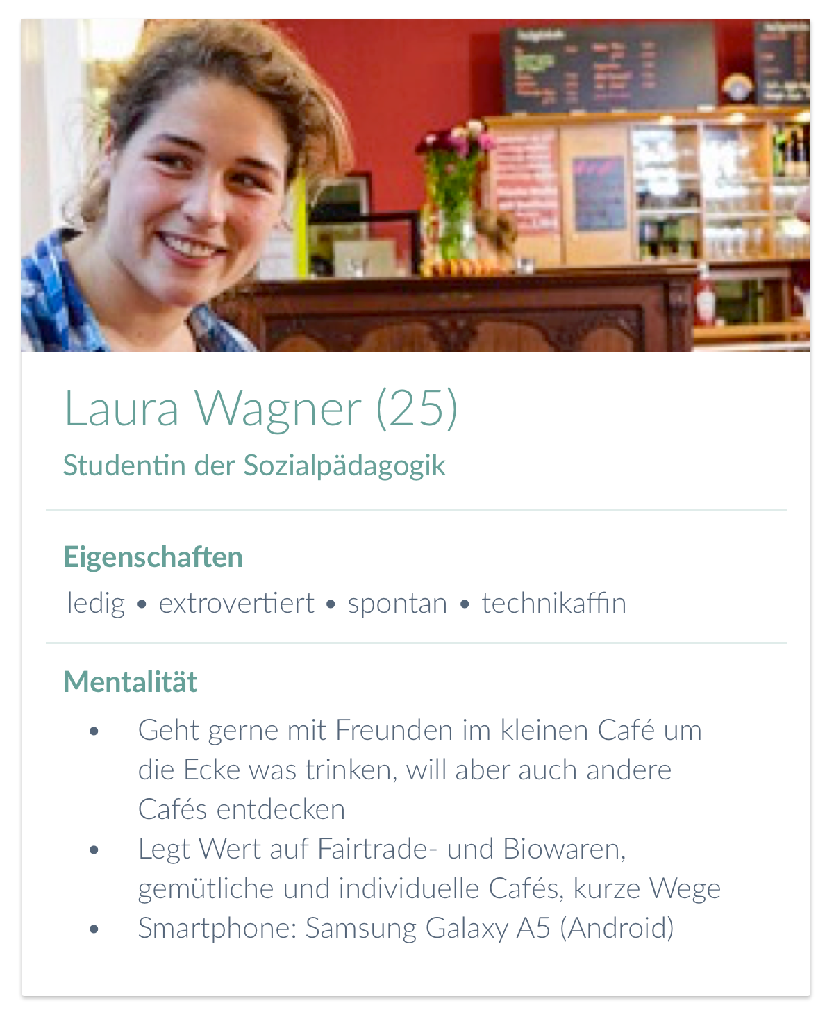
\includegraphics[width=0.5\textwidth]{Bilder/laura.eps}
		\caption{Primärpersona Laura Wagner}
\end{figure}

\subsection{Sekundärpersona}
Roland Reisenweber vertritt die sekundäre Zielgruppe. Er...
\begin{itemize}
	\item ...ist 42 Jahre alt
	\item ...verheiratet
	\item ...arbeitet als Journalist bei Frankfurter Allgemeine
	\item ...ist extrovertiert und offen für Neues
	\item ...arbeitet gerne an öffentlichen Orten
	\item ...besitzt ein ausgeprägtes soziales Bewusstsein
	\item ...ist gerne mit seiner Frau auf Reisen (innerhalb der EU)
	\item ...will regionale Kulturen kennenlernen
	\item ...ist weniger technikaffin, d. h. er nutzt sein iPhone nur zum telefonieren
\end{itemize}

\begin{figure}[h!]
    \centering
		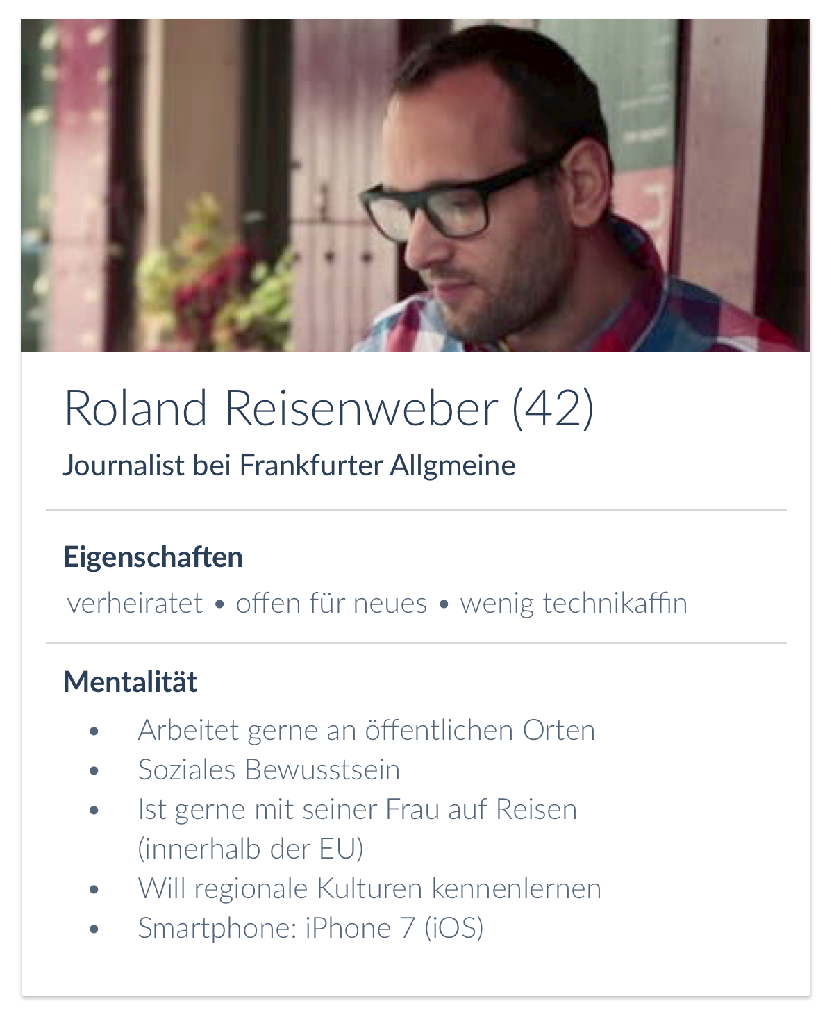
\includegraphics[width=0.5\textwidth]{Bilder/roland.eps}
		\caption{Sekundärpersona Roland Reisenweber}
\end{figure}

\section{Anforderungsanalyse}
In der Anforderungsanalyse haben wir die Muss-, Soll- und Kann-Anforderungen von comfycoffee definiert.

\subsection{Muss-Anforderungen}
\label{subsec:mussanforderungen}
Die Muss-Anforderungen wurden auf das Nötigste heruntergebrochen, um die App sinnvoll bedienen zu können. Vorgabe war, den Bewegungssensor (Gyroskop) und GPS zu benutzen. Daraus ergaben sich die folgenden Muss-Anforderungen:

\begin{itemize}
	\item Lokale Cafés in der Nähe anzeigen
	\item Kartenansicht in Google Maps
	\item Listenansicht
	\item Standortdaten via Google API
	\item Kaffeelexikon
	\item Einträge über Zubereitungsarten
	\item Schüttelfunktion (Benutzung des Bewegungssensors) für Zufallswahl einer Zubereitungsart
\end{itemize}

\subsection{Soll-Anforderungen}
Die Soll-Anforderungen erweitern den Funktionsumfang der App um nützliche Inhalte. Diese waren:

\begin{itemize}
	\item Navigation zu ausgewähltem Café über die App \emph{Google Maps}
	\item Listenansicht mit den wichtigsten Standortinformationen
	\item Detailseite mit mehr Infos über das Café (die Informationen sind abhängig davon, was die Google API zur Verfügung stellt)
\end{itemize}

\subsection{Kann-Anforderungen}
Die Kann-Anforderungen ergänzen die App durch weitere Informationen und Features, die der Nutzer nicht zwingend erwartet, aber als angenehm empfindet. Die Kann-Anforderungen waren:

\begin{itemize}
	\item Mehr Daten über zusätzliche APIs
	\item Eigene Bewertungen der Cafés durch die App
	\item Eigene Standorte vorschlagen
	\item Erweitertes Lexikon (z. B. mit Kaffeesorten, etc.)
	\item Profil des Nutzers anlegen
\end{itemize}

\underline{Learnings:}
Dabei war die Herausforderung, die Anforderungen exakt zu formulieren und in Pakete zu unterteilen, die klein genug waren, um sie in der im Ablaufplan definierten Zeit abzuarbeiten (vgl. Kapitel \ref{sec:ablaufplan}).

\section{Ablaufplan}
\label{sec:ablaufplan}
Anschließend wurde ein Ablaufplan ausgearbeitet und festgelegt. Dabei sollte die Designphase mit Wireframes, Flow Charts, Mockups und einem interaktiven Prototyp bis zum 22.11.2017 abgeschlossen sein. Für die Einarbeitung in das Entwicklungsframework, React Native (vgl. Kapitel \ref{sec:reactnative}), wurde eine Woche eingeplant. Bis zum 29.11.2017 sollte eine ``Hello World''-Anwendung laufen, um die Grundzüge des Frameworks zu beherrschen. Zwei Wochen, also bis zum 13.12.2017, waren für die Muss-Anforderungen, eine Woche für die Soll-Anforderungen (bis 20.12.2017) geplant. Die Kann-Anforderungen sollten im Januar 2018 abgeschlossen sein. Das folgende Diagramm veranschaulicht den Ablauf.

\begin{figure}[h!]
    \centering
		
\includegraphics[width=\textwidth]{Bilder/ablaufplan.png}
		\caption{Ablaufplan der Konzeption und Entwicklung von comfycoffee}
\end{figure}

\underline{Learnings:}
Die Aufwandsschätzung zu Beginn gestaltete sich als schwierig, da keine Erfahrung mit React Native und der Cross-Plattform-Entwicklung bzw. allgemein der App-Entwicklung vorhanden war.

\section{Flow Chart}
Das Flow Chart stellt die Navigation durch die App und die verschiedenen Views dar. Von der Startseite aus kann der Nutzer wählen, ob er die Karte mit den Cafés in der Nähe oder das Kaffee-Lexikon aufrufen will.

In der Karte befindet sich eine Bottom Navigation Bar, mit der von der Karte zur Listenansicht und zurück gewechselt werden kann. Klickt der Nutzer in der Karte auf einen Marker oder in der Liste auf einen Eintrag, so wird er auf die Detailseite des jeweiligen Café geleitet. Dort erhält er Informationen wie Adresse, Öffnungszeiten und Bewertungen des Cafés. Über einen Button wird die Navigation zu dem Café in Google Maps geöffnet. Das Navigationskonzept wurde in der Entwicklung abgeändert, um den Design-Guidelines von Android und iOS zu entsprechen. Aus der Bottom Navigation Bar wurde in Android eine Tab Bar. Weiterhin wird auf der Detailseite eine Tab bzw. Bottom Navigation Bar angezeigt, um von der Seite des Cafés zu den Bewertungen zu wechseln.

Das Lexikon beinhaltet verschiedene Kaffeesorten. Beim Auswählen einer Kaffeesorte wird der Nutzer auf eine Unterseite geleitet, die Details zu der jeweiligen Kaffeesorte enthält. Schüttelt der Nutzer das Smartphone, während er sich auf der Übersichtsseite des Lexikons befindet, wird zufällig eine Kaffeesorte ausgewählt und der Nutzer hat die Möglichkeit, sich zu der genannten Detailseite navigieren zu lassen.

\begin{figure}[h!]
    \centering
		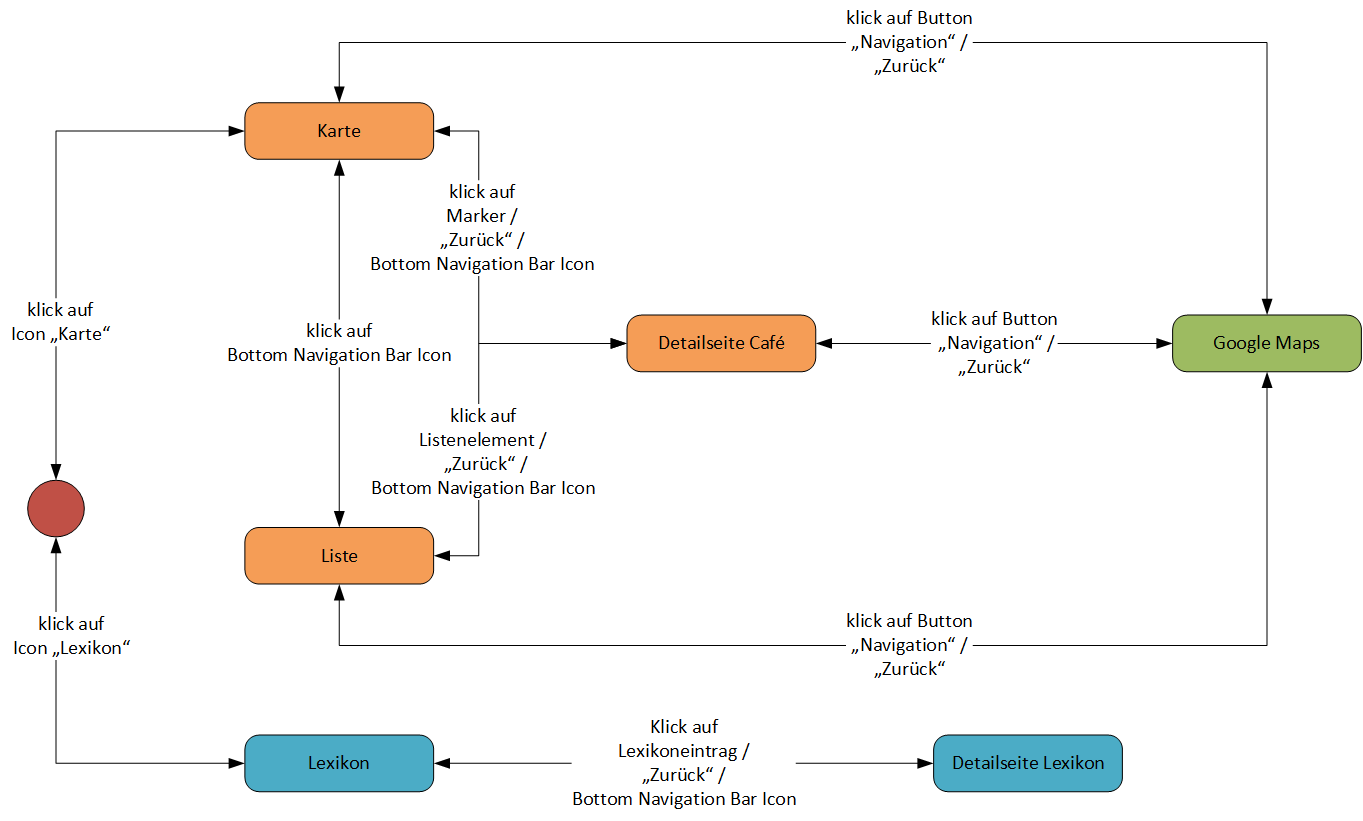
\includegraphics[width=\textwidth]{Bilder/flowchart.png}
		\caption{Erster Entwurf des Flow Charts von comfycoffee}
\end{figure}

\section{Wireframes}
Nachdem die Anzahl und Anforderungen an die Views feststanden, wurden diese auf Papier in Form von Wireframes visualisiert. Dabei wurden die Elemente pro View bestimmt und deren Position auf den einzelnen Seiten festgelegt.
Bilder rein???

\section{Mockups}
Aus den Wireframes wurden Mockups mit dem Mockup-Tool Axure konfiguriert. Zu jeder View wurde ein Mockup erstellt. Im Gegensatz zu den Wireframes sind hier schon Farben, Bilder und Texte beispielhaft enthalten.

\section{Prototyp}
Anhand der Mockups und des Flow Charts wurde in Axure ein interaktiver Prototyp erstellt. Er dient zum Durchklicken durch die App und um einen ersten Eindruck in Sachen Usability zu gewinnen.

\begin{figure}[h!]
    \centering
		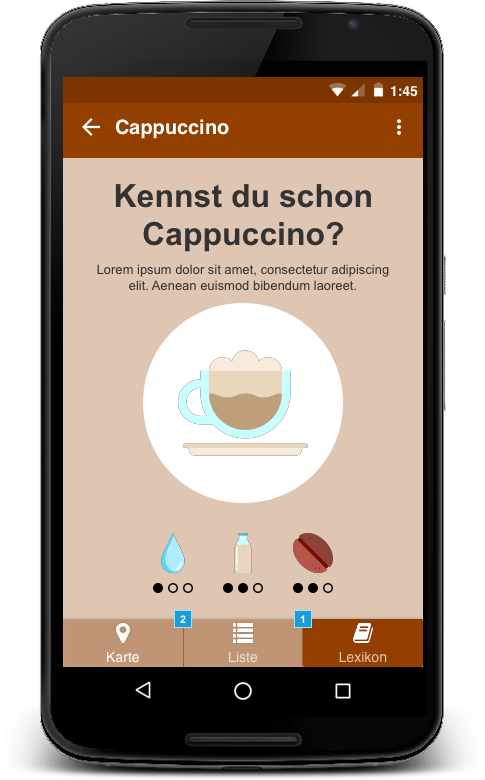
\includegraphics[width=0.5\textwidth]{Bilder/detail.png}
		\caption{Ansicht der Detailseite eines Kaffees im interaktiven Prototyp von comfycoffee}
\end{figure}


\chapter{Entwicklung}
\label{entwicklung}
Mit dem Abschluss der Konzeptionsphase begann die technische Umsetzung der App.
Nachdem ein passendes Framework zur Entwicklung der App auf mehreren Plattformen gefunden wurde konnte eine sinnolle Projektstruktur mit allen benötigten Bibliotheken angelegt werden.
Die Implementierung einiger Freatures wurde dabei parallel durchgeführt.
Weiterhin wird in diesem Kapitel der aktuelle Stand der App beschrieben.
Eine Readme inklusive Installationsanleitung schließt die technische Seite des Projekts ab.



\section{React Native}
\label{sec:reactnative}
Nach kurzer Diskussion und dem Abwägen von Vor- und Nachteilen entschieden wir uns das \emph{React Native} Framework zu benutzen.
React Native stellt somit das technische Kernelement des Projekts dar.
Als ein von \emph{Facebook} entwickeltes und verwaltetes Repository erfreut es sich mit über 58.000 Sternen auf \emph{GitHub} großer Beliebtheit.
Demnach steht bereits eine große Community hinter dem Cross-Plattform-Framework.
Die Entwicklung mit React Native erfolgt fast ausschließlich über JavaScript.
Als Cross-Plattform-Framework ermöglicht React Native den Zugriff auf native Komponenten via JavaScript und profitiert somit von einer besseren Performance als hybride Frameworks.
Allerdings erscheint es trotz seiner Popularität technisch noch nicht sehr etabliert.
Darüber hinaus benötigen die nativen Komponenten meist noch Anpassungen per Hand für Android und iOS.



\section{Setup}
Um React Native einem Projekt hinzuzufügen stehen zwei Möglichkeiten zur Verfügung.
Eine davon ist der \emph{Quick Start}, welcher nach erfolgreichem Ausführen einen QR-Code anzeigt.
Über das Smartphone kann der Code gescannt und die App aufgerufen werden.
Vor- und Nachteil gleichermaßen ist, dass die Entwicklungsumgebungen \emph{Android Studio} für Android und \emph{Xcode} für iOS nicht installiert sein müssen.
Allerdings ist es somit auch nicht möglich, selbsterstellte React Native Module hinzuzufügen.
Demnach entschieden wir uns für die zweite Variante, um zusätzlich Zugriff auf eigene Module zu haben.
Hierbei wird React Native über die Kommandozeile und den Befehl 'create-react-native-app' initialisiert.
\\
Grundvoraussetzungen hierbei sind eine funktionierende Version von \emph{Node.js} sowie das Facebook Tool \emph{Watchman}.
Für die Verwaltung von Abhängikeiten wird bei der Installation von React Native der Paketmanager \emph{Yarn} hinzugefügt, der Zugriff auf die über den \emph{Node Package Manager (npm)} bereitgestellten Module ermöglicht.
Zusätzlich müssen die beiden Entwicklungsumgebungen Android Studio und Xcode zum Kompilieren des nativen Codes bereit stehen.
Testing und Debugging der App kann somit entweder über die in Android Studio und Xcode integrierten Simulatoren erfolgen oder aber direkt über ein verbundenes Smartphone.
\\
Unsere Wahl für einen Code Editor fiel auf \emph{Visual Studio Code} von Microsoft, da es einen einfachen Einstieg bietet und sowohl für Windows als auch für Mac verfügbar ist.
Als Versionierungssystem benutzten wir Bitbucket, welches die Verwaltung von Git-Repositories ermöglicht.
Des Weiteren richteten wir ein \emph{Trello-Board} ein, auf dem das Projektmanagement abgebildeten werden sollte.
\\
\underline{Learnings:}
Obwohl die Konzeption unserer App auf einen eher geringen Umfang schließen lässt wurden doch sehr viele Tools benötigt, um eine Entwicklung zu ermöglichen.
Für diese Projektgröße stellte sich auch das Projektmanagementtool Trello als zu aufwändig in der Pflege heraus.



\section{Module}
Für die Implementierung einiger Funktionalitäten stehen bereits zahlreiche Komponenten und Pakete aus der Community zu Verfügung.
Zusätzlich zu den bereits in React Native integrieren Modulen werden folgende in der App verwendet:
\begin{itemize}
	\item axios: erleichtert die Kommunikation mit beliebigen APIs, da es entsprechende Hilfmethoden zur Verfügung stellt.
	\item react-native-maps: eine benutzerdefinierte React Native Komponente, welche die Integration einer Google Maps Karte ermöglicht. Leider ein sehr undokumentiertes Module, welches große Probleme bei der Integration aufwirft.
	\item react-native-permissions: bietet eine Schnittstelle zur Abfrage von unterschiedlichen Berechtigungen, beispielsweise dem Zugriff auf den aktuellen Standort.
	\item react-native-sensors: ermöglicht den direkten Zugriff auf den Bewegungssensor des entsprechenden Endgeräts - leider ein ebenfalls eher undokumentiertes Modul.
	\item react-native-star-rating: die visuelle Darstellung eines Werts (wie beispielsweise einer Bewertung) in Form von Sternen verpackt in einer React Native Komponente.
	\item react-native-vector-icons: eine Sammlung thematisch geordneter Icon-Bibliotheken, welche nach dem Import direkt zur Verfügung stehen.
	\item react-navigation: ein alternatives Navigationskonzept als React Native Modul aus der Community. Dieses ersetzt das in React Native integrierte Konzept und ermöglicht eine einfache Implementierung diverser Navigationselemente.
\end{itemize}
Während der Entwicklung wurden einige zusätzliche Module eingebunden, welche allerdings nicht den gewünschten Anforderungen entsprachen:
\begin{itemize}
	\item react-native-material-bottom-navigation: die ebenfalls in den Material Design Guidelines vertretene Bottom Navigation für Android verpackt in einer React Native Komponente. In dieser App wird allerdings die Navigation in Android über Tabs bevorzugt.
	\item react-native-stars: eine Alternative zu dem verwendeten react-native-star-rating Modul. Da dieses Modul weniger Konfigurationsmöglichkeiten bietet als sein Pendant ist es obsolet.
	\item react-native-google-places-autocomplete: die reduzierte Variante des react-native-maps Moduls. Allerdings ist der Funktionsumfang deutlich zu gering, so bietet es lediglich autocomplete für die Google Places API.
\end{itemize}
Durch die zahlreichen verfügbaren Komponenten lässt sich eine React Native App sehr stark modularisieren.
Es können bei Bedarf die jeweils benötigen Funktionalitäten isoliert angefordert und eingebunden werden.
Einzig undokumentierte und redundante Module stellen einen zusätzlichen Aufwand dar.
Diese müssen zunächst herausgefiltert und getestet werden, um die beste Lösung zu finden.



\section{Arbeitsaufteilung}
Die Aufteilung der anstehenden Aufgaben sahen wir als notwendig an, um die geplanten Deadlines einhalten zu können.
Unumgänglich war allerdings eine gemeinsame Code-Basis, in die zusätzliche Funktionalitäten unabhängig voneinander integriert werden konnten.
Hierzu legten wir durch \emph{Pair Programming} zusammen eine geeignete Grundlage.

\subsection{Gemeinsam}
Das Fundament besteht aus dem Grundgerüst der App sowie der Navigation durch diese.
Dabei besteht das Navigationskonzept aus einer übergeordneten \emph{Stack Navigation} sowie mehreren kontextabhängigen, verschachtelten \emph{Tab/Bottom Navigations}.
Eine dem Flow Chart entsprechende Seitenstruktur ermöglicht es, Seiteninhalte isoliert zu bearbeiten.
Die Implementierung der Karte wurde ebenfalls gemeinsam gelöst, allerdings nach Betriebssystemen getrennt.
Sobald der Rahmen der App aufgebaut war arbeiteten wir an unterschiedlichen Funktionalitäten weiter.
\\
\underline{Learnings:}
Bereits in diesem frühen Stadium konnten wir einige Aha-Momente für uns entdecken.
Die Tabs und Bottom Navigation, so wie in unseren MockUps skizziert, ließ sich nur teilweise realisieren.
Eine weitere Recherche ergab, dass der Aufbau der Navigation in React Native eine andere Lösung für diesen Fall vorgab und wir die Implementierung entsprechend anpassen mussten.
Darüber hinaus stießen wir mit dem React Native Modul für die Google Maps Karte (react-native-maps) bereits auf ein undokumentiertes Modul aus der Community, welchem noch weitere folgen sollten.

\subsection{Katharina}
Die Umsetzung der Inhalte des Lexikons und der Lexikon-Detailansicht sowie die Integration des Bewegungssensors übernahm Katharina Garrecht.
Hierbei implementierte sie die im Prototypen definierten Elemente sowohl für die Übersichtsseite als auch für das Template der Kaffee-Detailseite.
Die Detailseiten werden dabei mit in einer JSON Datei hinterlegten Inhalten gespeist.
Auf der Übersichtsseite selbst ist der Bewegungssensor aktiv, welcher bei Erkennung einer Schüttelgeste zufällig eine der zur Verfügung stehenden Kaffee-Zubereitsungsarten auswählt und vorschlägt.
\\
\underline{Learnings:}
Die Integration des Bewegungssensors in die bestehende Navigation brachte einige Stolpersteine mit sich, die nur durch lange Recherchen und Umwege überwunden werden konnten.
Auch die Einarbeitung in native UI Komponenten der jeweiligen Betriebssysteme war für die Umsetzung dieser Funktionalitäten notwendig.

\subsection{Thomas}
Die Darstellung der Listenansicht aller nahen Cafés sowie die Detailansicht einzelner Cafés fiel in den Aufgabenbereich von Thomas Wedler.
Ebenso Teil dieses Bereichs war die Implementierung der Geolocation zur Ermittlung des aktuellen Standorts.
Über diese Geokoordinaten werden bei Bedarf die \emph{Google Places API} und auch die \emph{Google Maps API} angesprochen.
Das Ergebnis ist situationsabhängig entweder eine Liste aller umliegenden Cafés mit rudimentären Informationen zu diesen oder aber ein ausführliches Objekt mit zahlreichen Detailinformationen über ein einzelnes Café.
\\
\underline{Learnings:}
Für die Umsetzung der benötigen Funktionalitäten war eine intensive Einarbeitung in das Ecosystem sowie die bereitgestellten Schnittstellen der Google APIs unumgänglich.
Ebenfalls hier mussten native UI Komponenten der jeweiligen Betriebssysteme korrekt identifiziert und implementiert werden.

\newpage

\section{Vorstellung der App}
\nopagebreak

\begin{table}[h!]
	\hskip-0.2cm\begin{tabular}{p{0.5\textwidth}p{0.5\textwidth}}
		\multicolumn{2}{p{\textwidth}}{\subsection{Startseite}} \\
		\multicolumn{2}{p{\textwidth}}{Der Einstiegspunkt der App. Von dort aus ist die Navigation zur Umkreissuche oder zum Lexikon möglich.} \\
		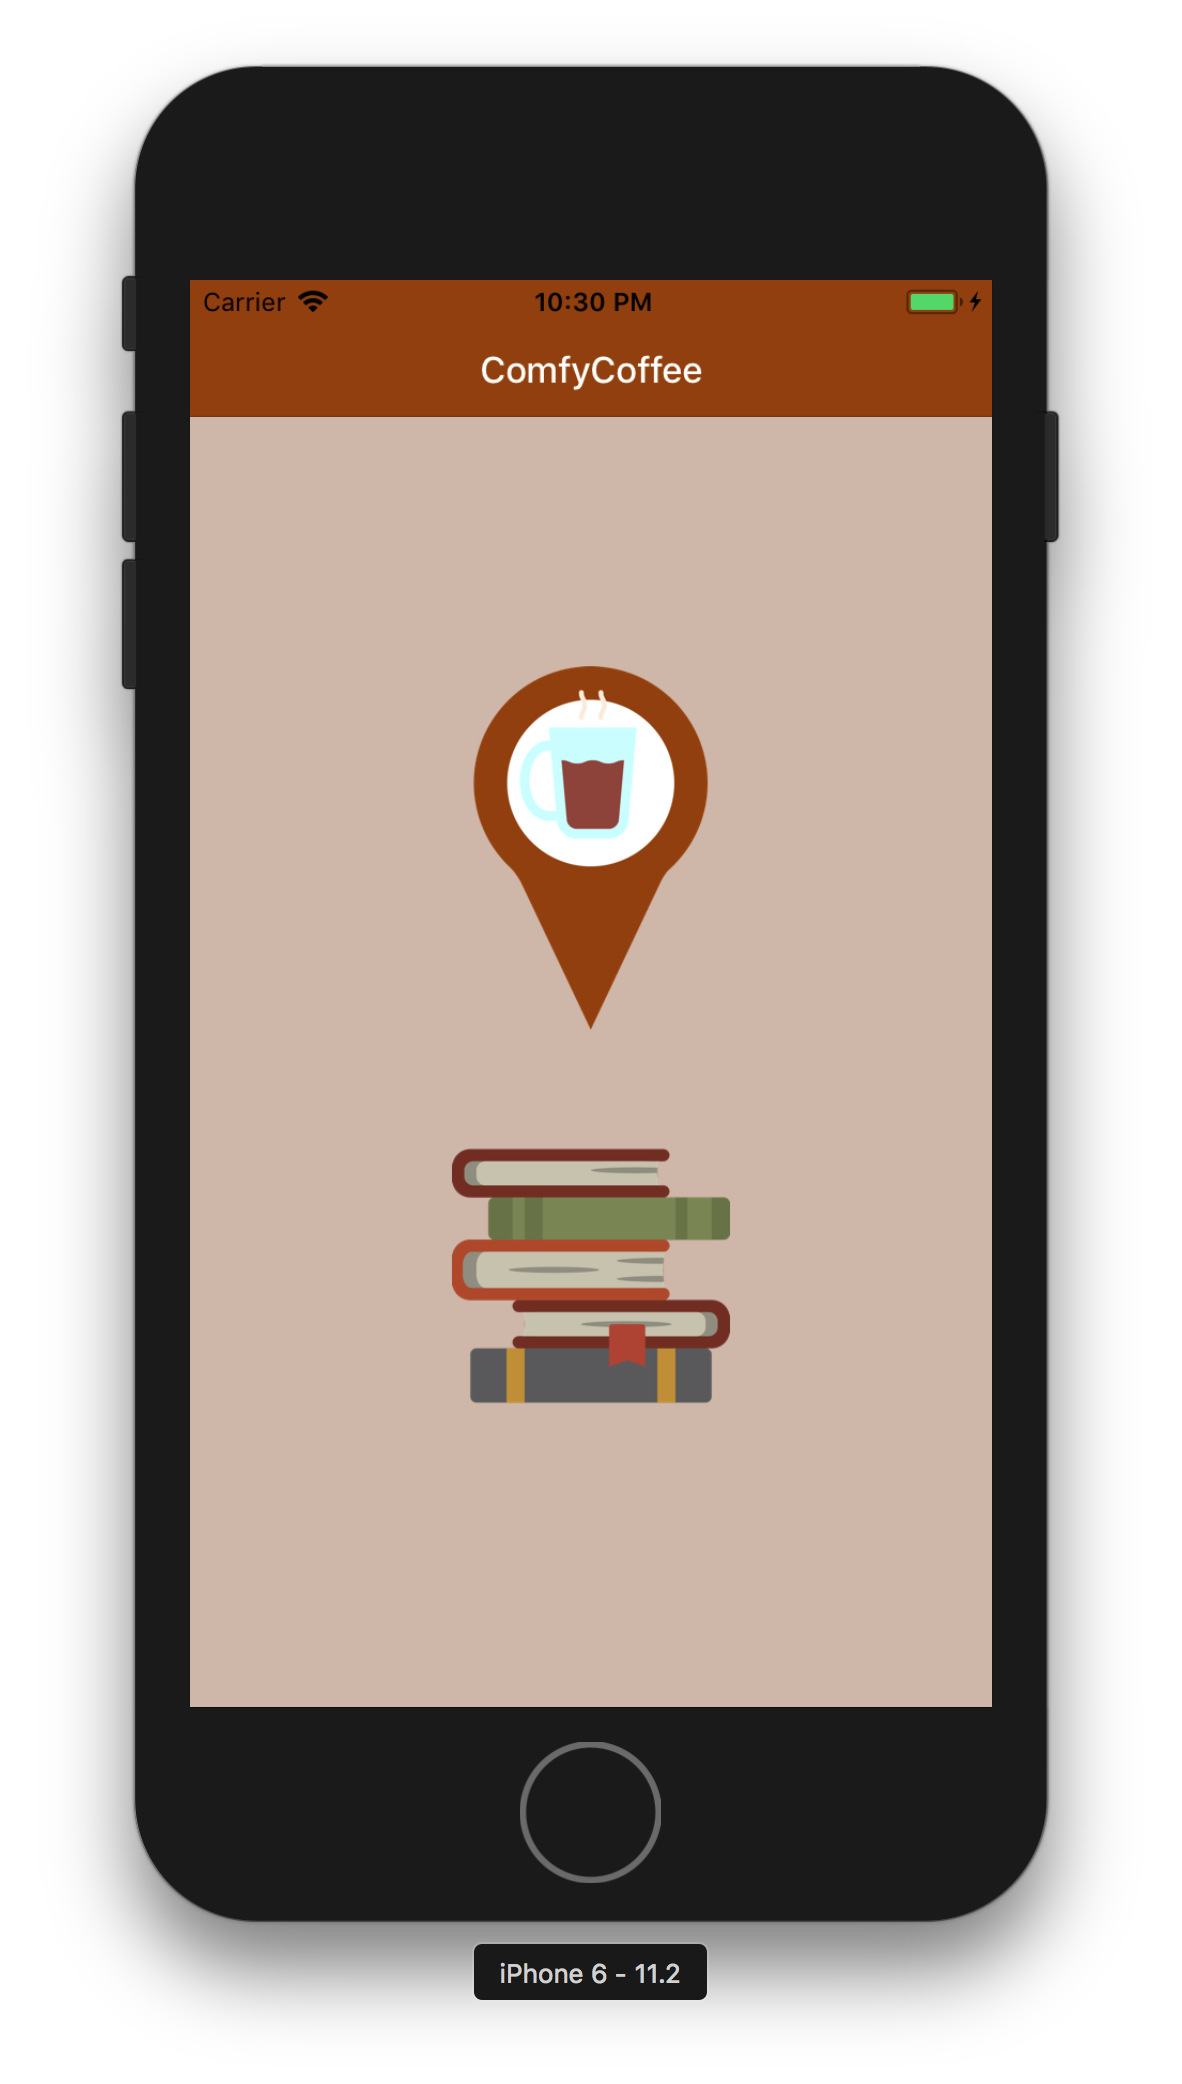
\includegraphics[width=0.5\textwidth]{Bilder/app-startseite.png}
		\captionof{figure}{Startseite der App unter iOS} &
		\centering
		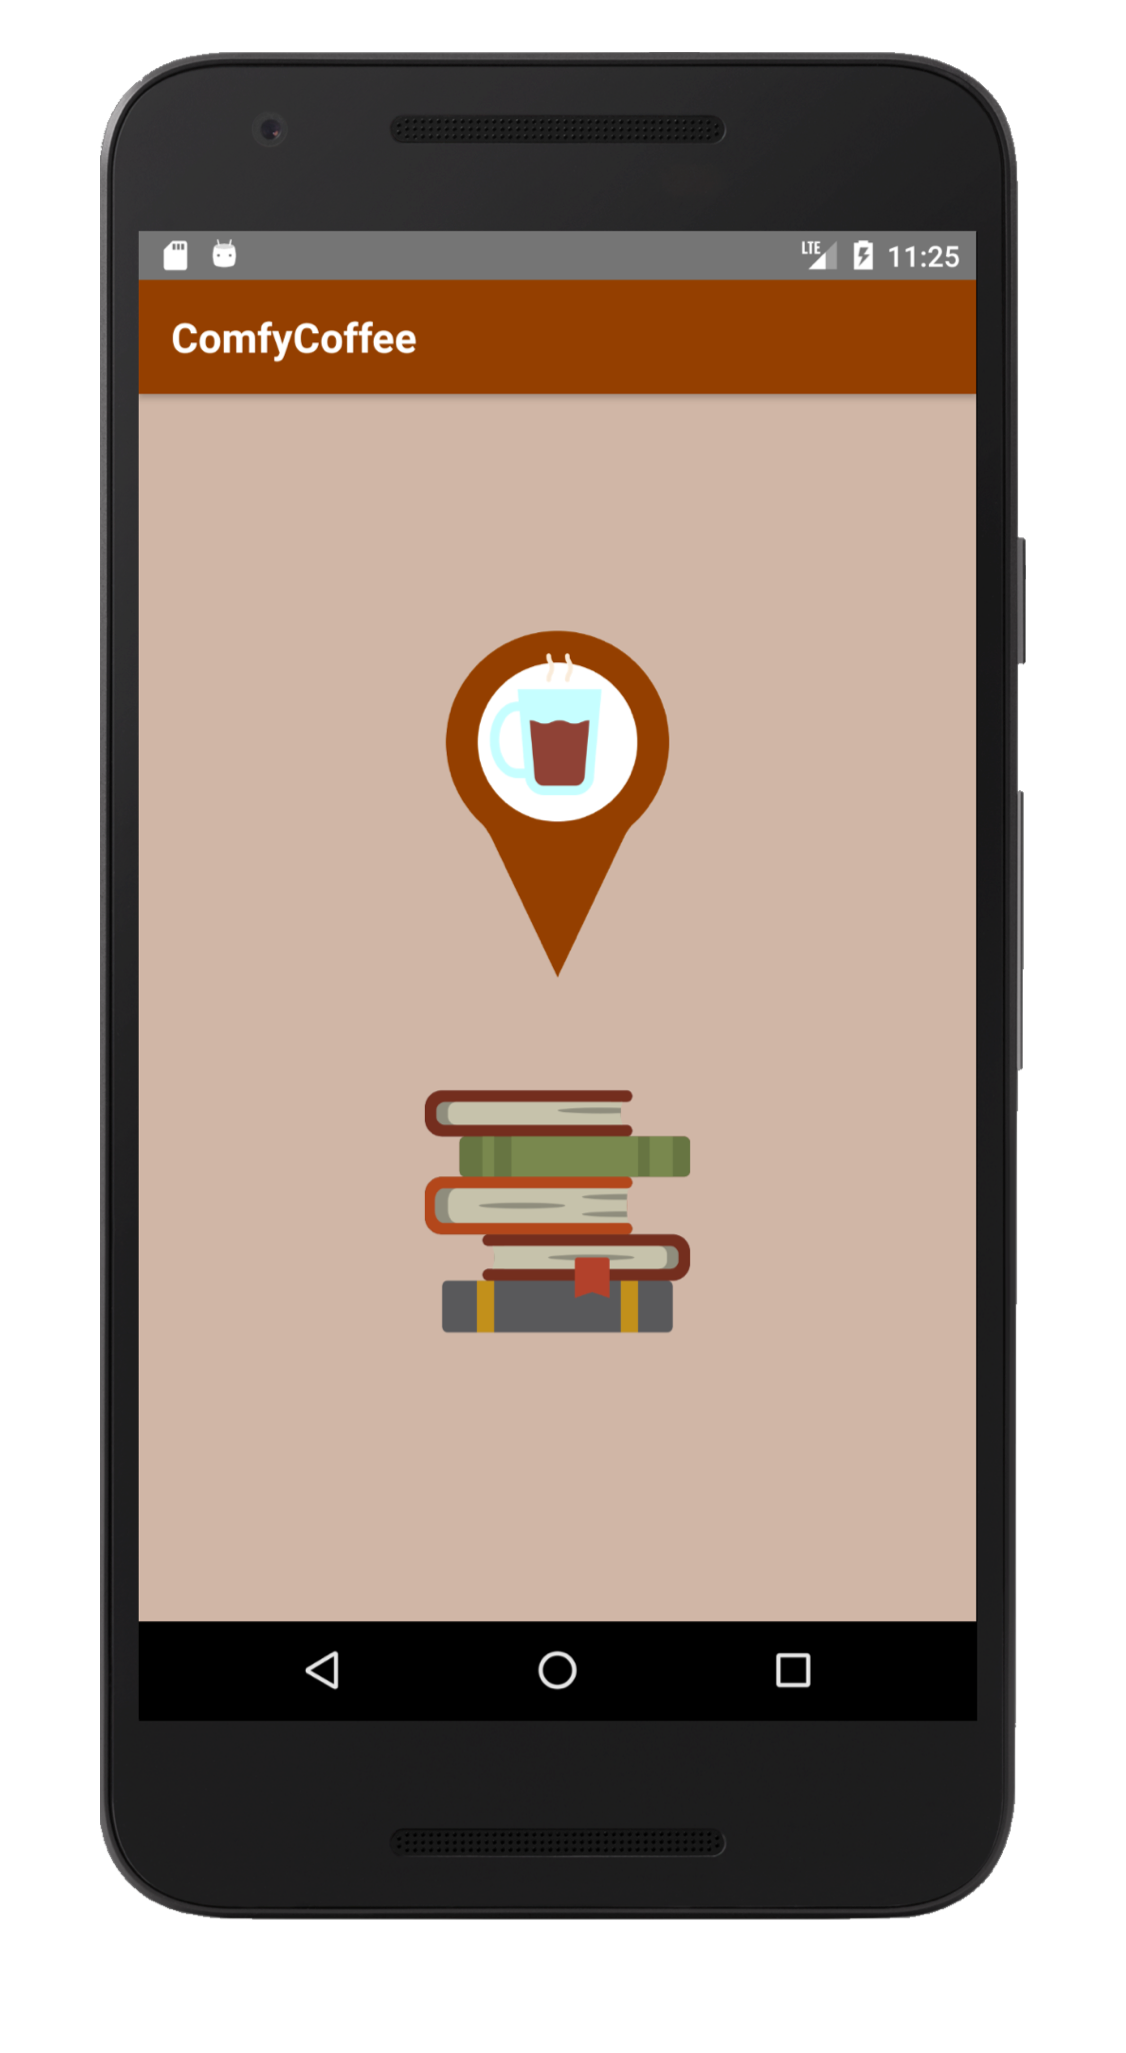
\includegraphics[width=0.5\textwidth]{Bilder/app-startseite_android.png}
		\captionof{figure}{Startseite der App unter Android}
	\end{tabular}
\end{table}

\begin{table}
	\vskip-2.5cm\hskip-0.2cm\begin{tabular}{p{0.5\textwidth}p{0.5\textwidth}}
		\multicolumn{2}{p{\textwidth}}{\subsection{Kartenansicht}} \\
		\multicolumn{2}{p{\textwidth}}{Hier werden auf einer interaktiven Google Maps Karte alle sich in der Nähe befindlichen Cafés einschließlich der aktuelle Standort angezeigt. Die hierfür benötigen Informationen werden über die entsprechenden Google APIs bezogen. Ein Klick auf einen Marker öffnet ein \emph{Bottom Sheet}, in welchem die wichtigsten Informationen über das ausgewählte Café wie etwa Entfernung, Bewertung, Öffnungszeiten oder Adresse angezeigt werden. Innerhalb dieses Sheets stehen Buttons zur Navigation auf die Detailseite des Cafés oder direkt zu Google Maps mit dem Café als hinterlegtem Ziel zur Verfügung. Des Weiteren erreicht man von hier aus über die Tab Navigation in Android sowie die Bottom Navigation in iOS die Listenansicht der angezeigten Cafés.} \\
		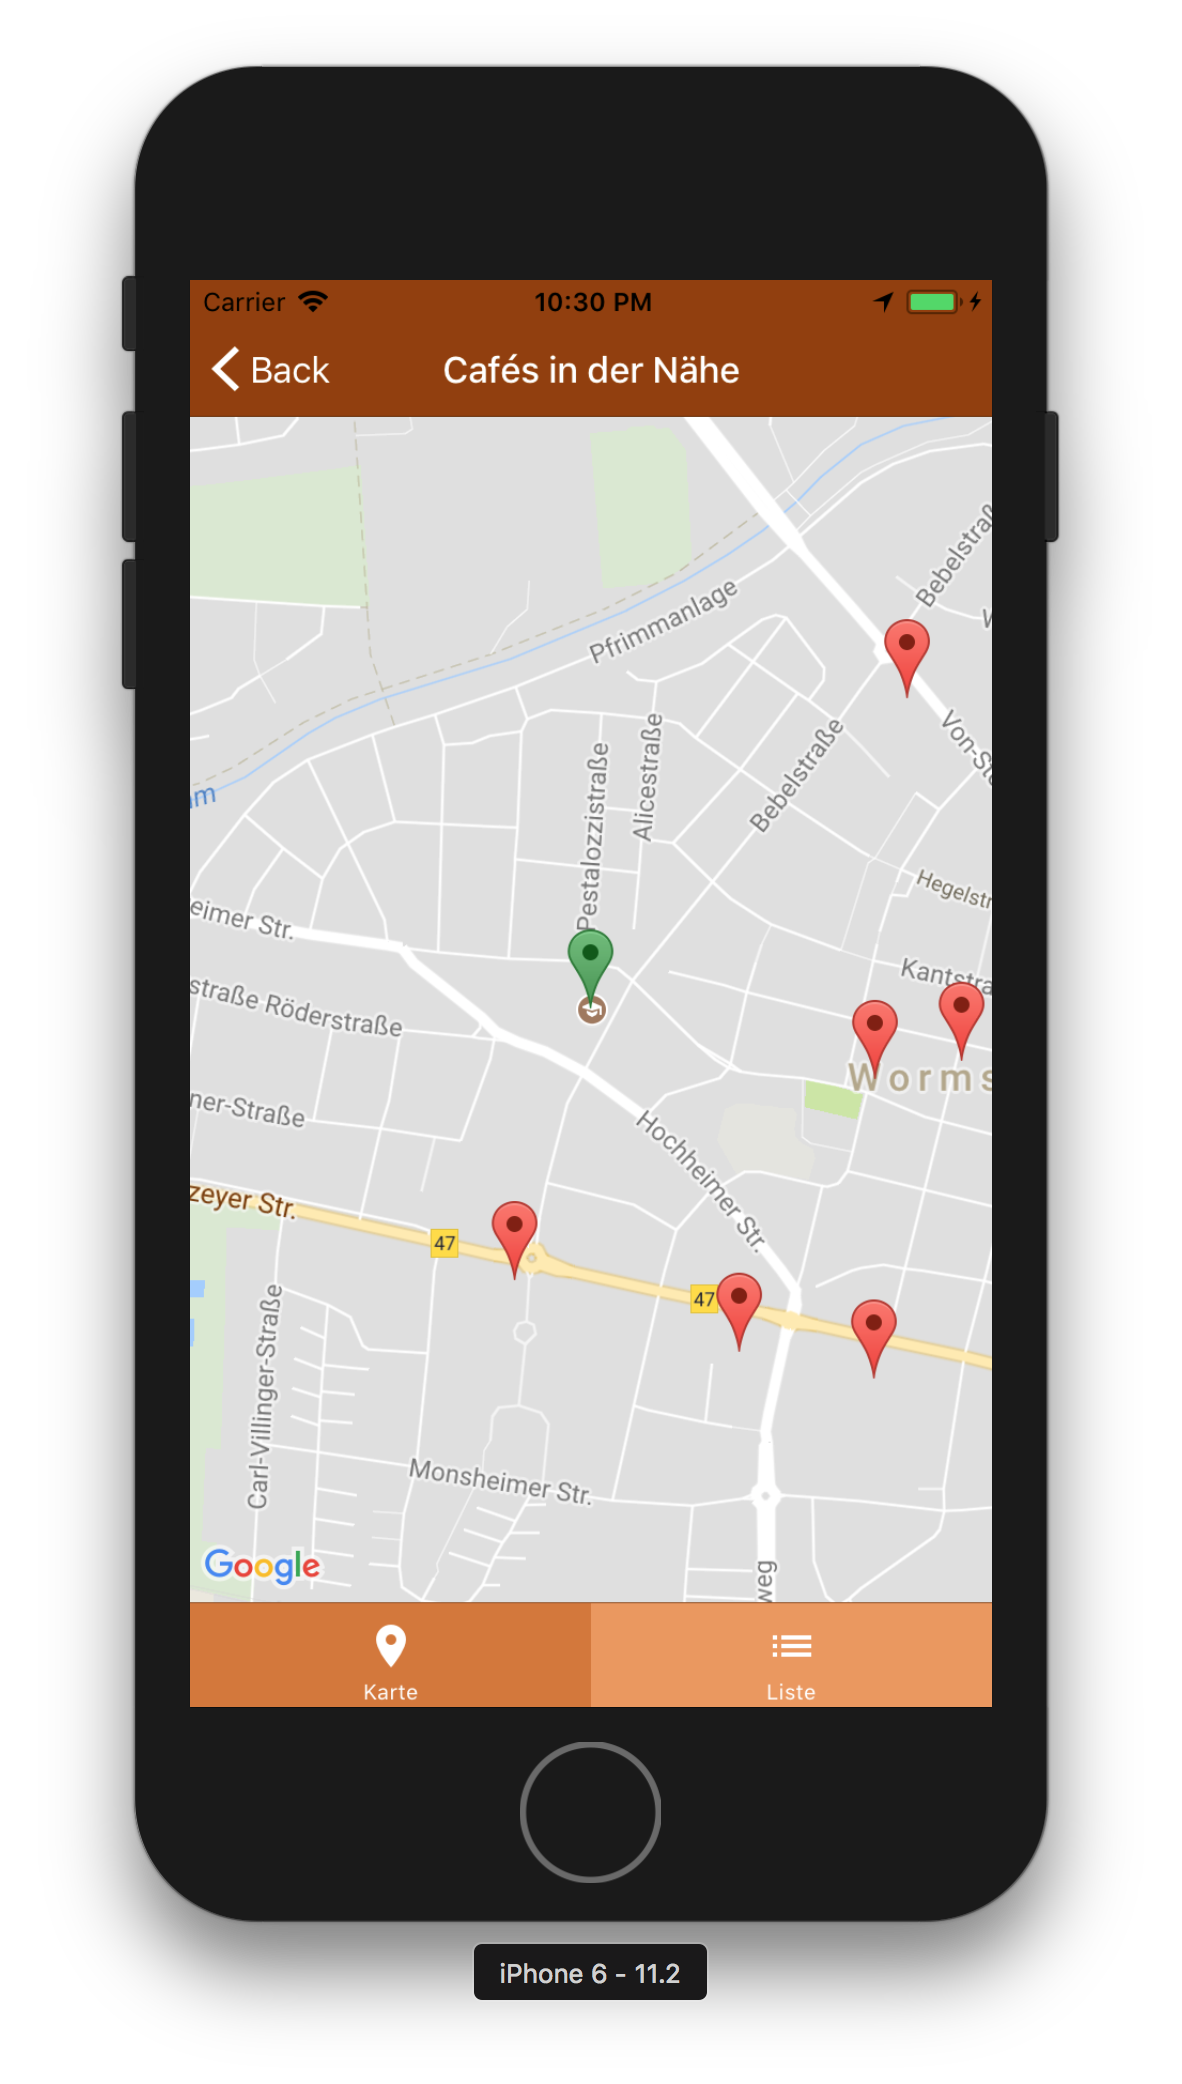
\includegraphics[width=0.5\textwidth]{Bilder/app-karte.png}
		\captionof{figure}{Kartenansicht der App unter iOS} &
		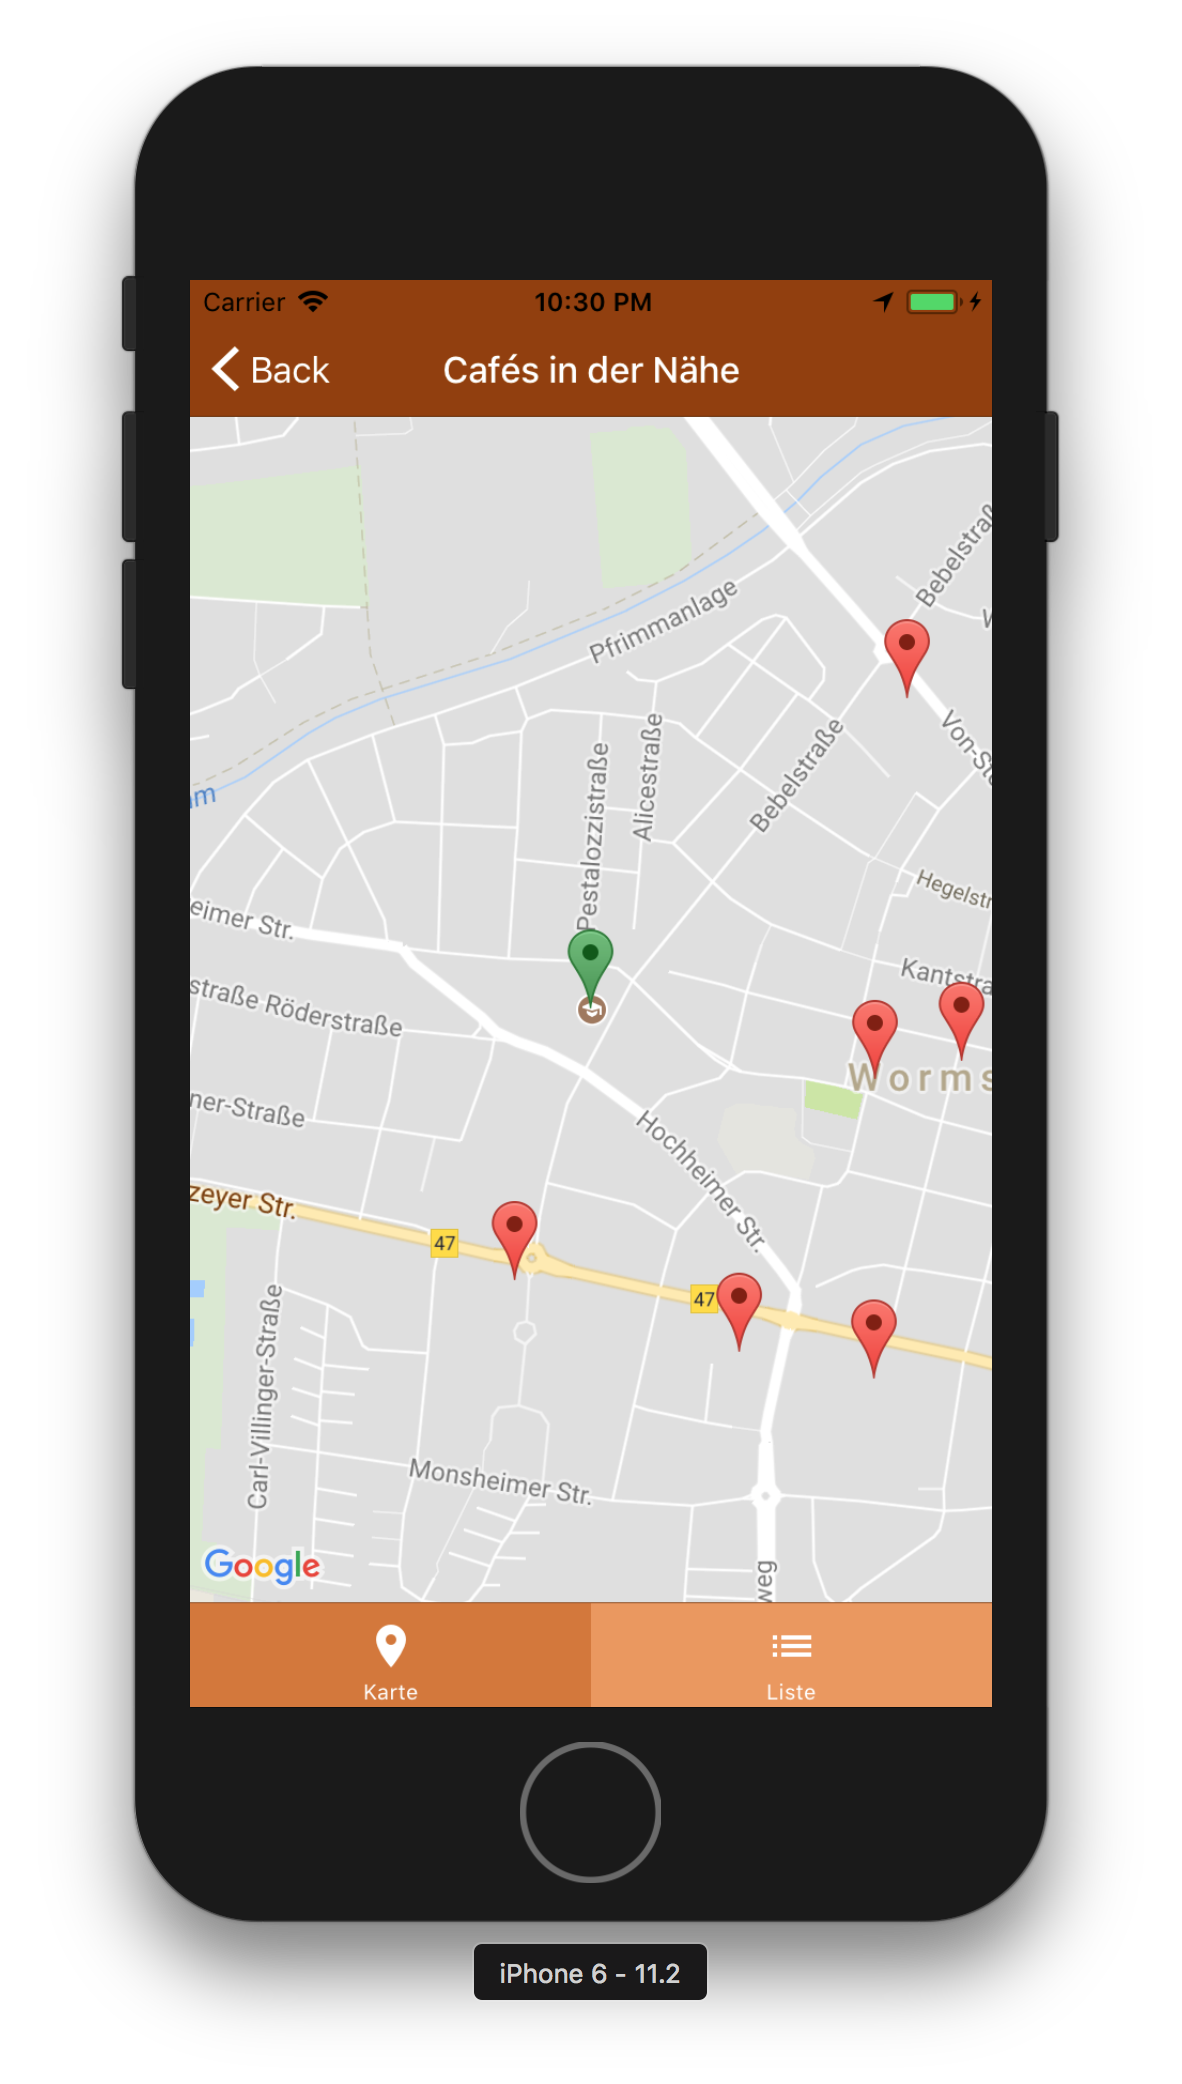
\includegraphics[width=0.5\textwidth]{Bilder/app-karte.png}
		\captionof{figure}{Kartenansicht der App unter Android}
	\end{tabular}
\end{table}

\begin{table}
	\vskip-3.5cm\hskip-0.2cm\begin{tabular}{p{0.5\textwidth}p{0.5\textwidth}}
		\multicolumn{2}{p{\textwidth}}{\subsection{Listenansicht}} \\
		\multicolumn{2}{p{\textwidth}}{Die bereits in der Kartenansicht dargestellten Standorte der Cafés werden hier in einer übersichtlichen Liste gezeigt. Jeder Listeneintrag enthält die gleichen Informationen und Interaktionsmöglichkeiten wie das Bottom Sheet aus der Karte, da es sich hierbei technisch um eine eigens konstruierte React Native Komponente handelt.} \\
		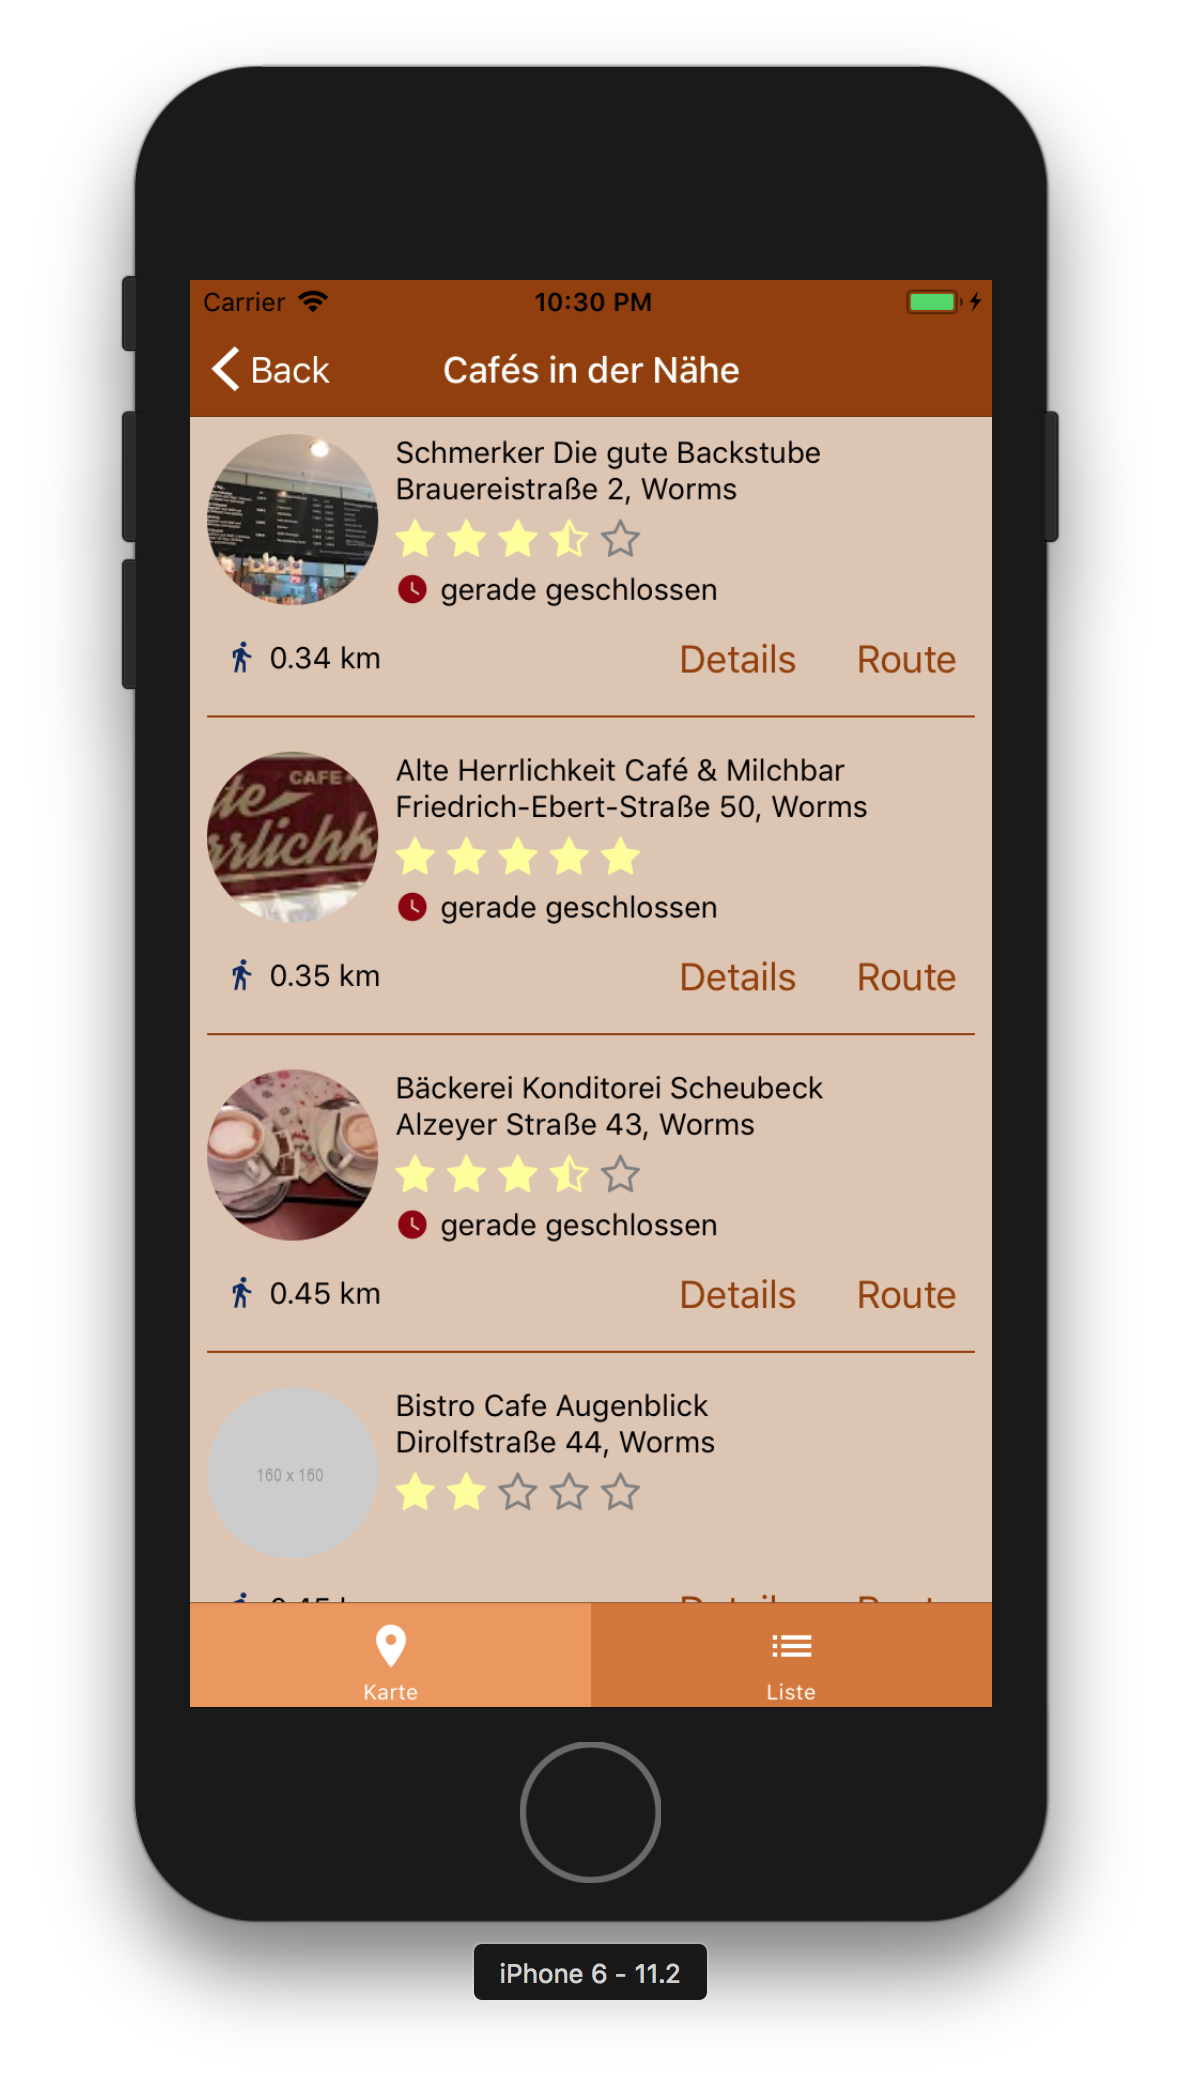
\includegraphics[width=0.5\textwidth]{Bilder/app-liste.png}
		\captionof{figure}{Listenansicht der App unter iOS} &
		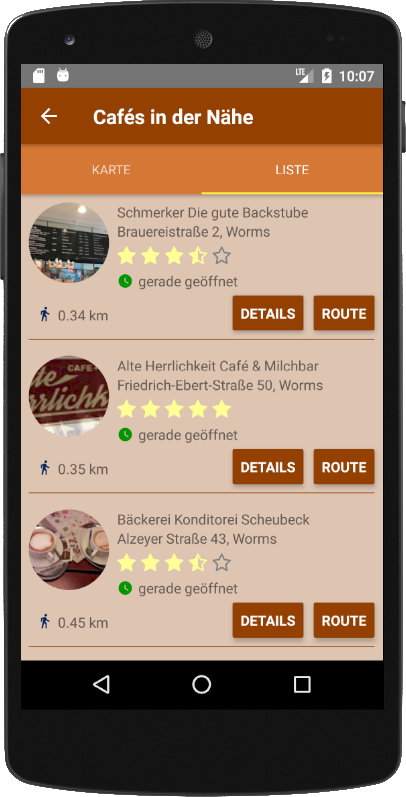
\includegraphics[width=0.5\textwidth]{Bilder/app-liste_android.png}
		\captionof{figure}{Listenansicht der App unter Android}
	\end{tabular}
\end{table}

\begin{table}
	\vskip-2.5cm\hskip-0.2cm\begin{tabular}{p{0.5\textwidth}p{0.5\textwidth}}
		\multicolumn{2}{p{\textwidth}}{\subsection{Infos Café}} \\
		\multicolumn{2}{p{\textwidth}}{Diese Seite zeigt die bereits im Bottom Sheet vorhandenen Informationen über das ausgewählte Café. Außerdem sind weitere Details wie Telefonnummer, Internetadresse oder auch Bilder des Cafés - soweit über die Google API bereit gestellt - verfügbar. Auch hier erreicht man über einen Button das Café als Zieladresse direkt in Google Maps. Darüber hinaus enthält die Tab Navigation respektive Bottom Navigation einen Link zur Bewertungsseite des Cafés.} \\
		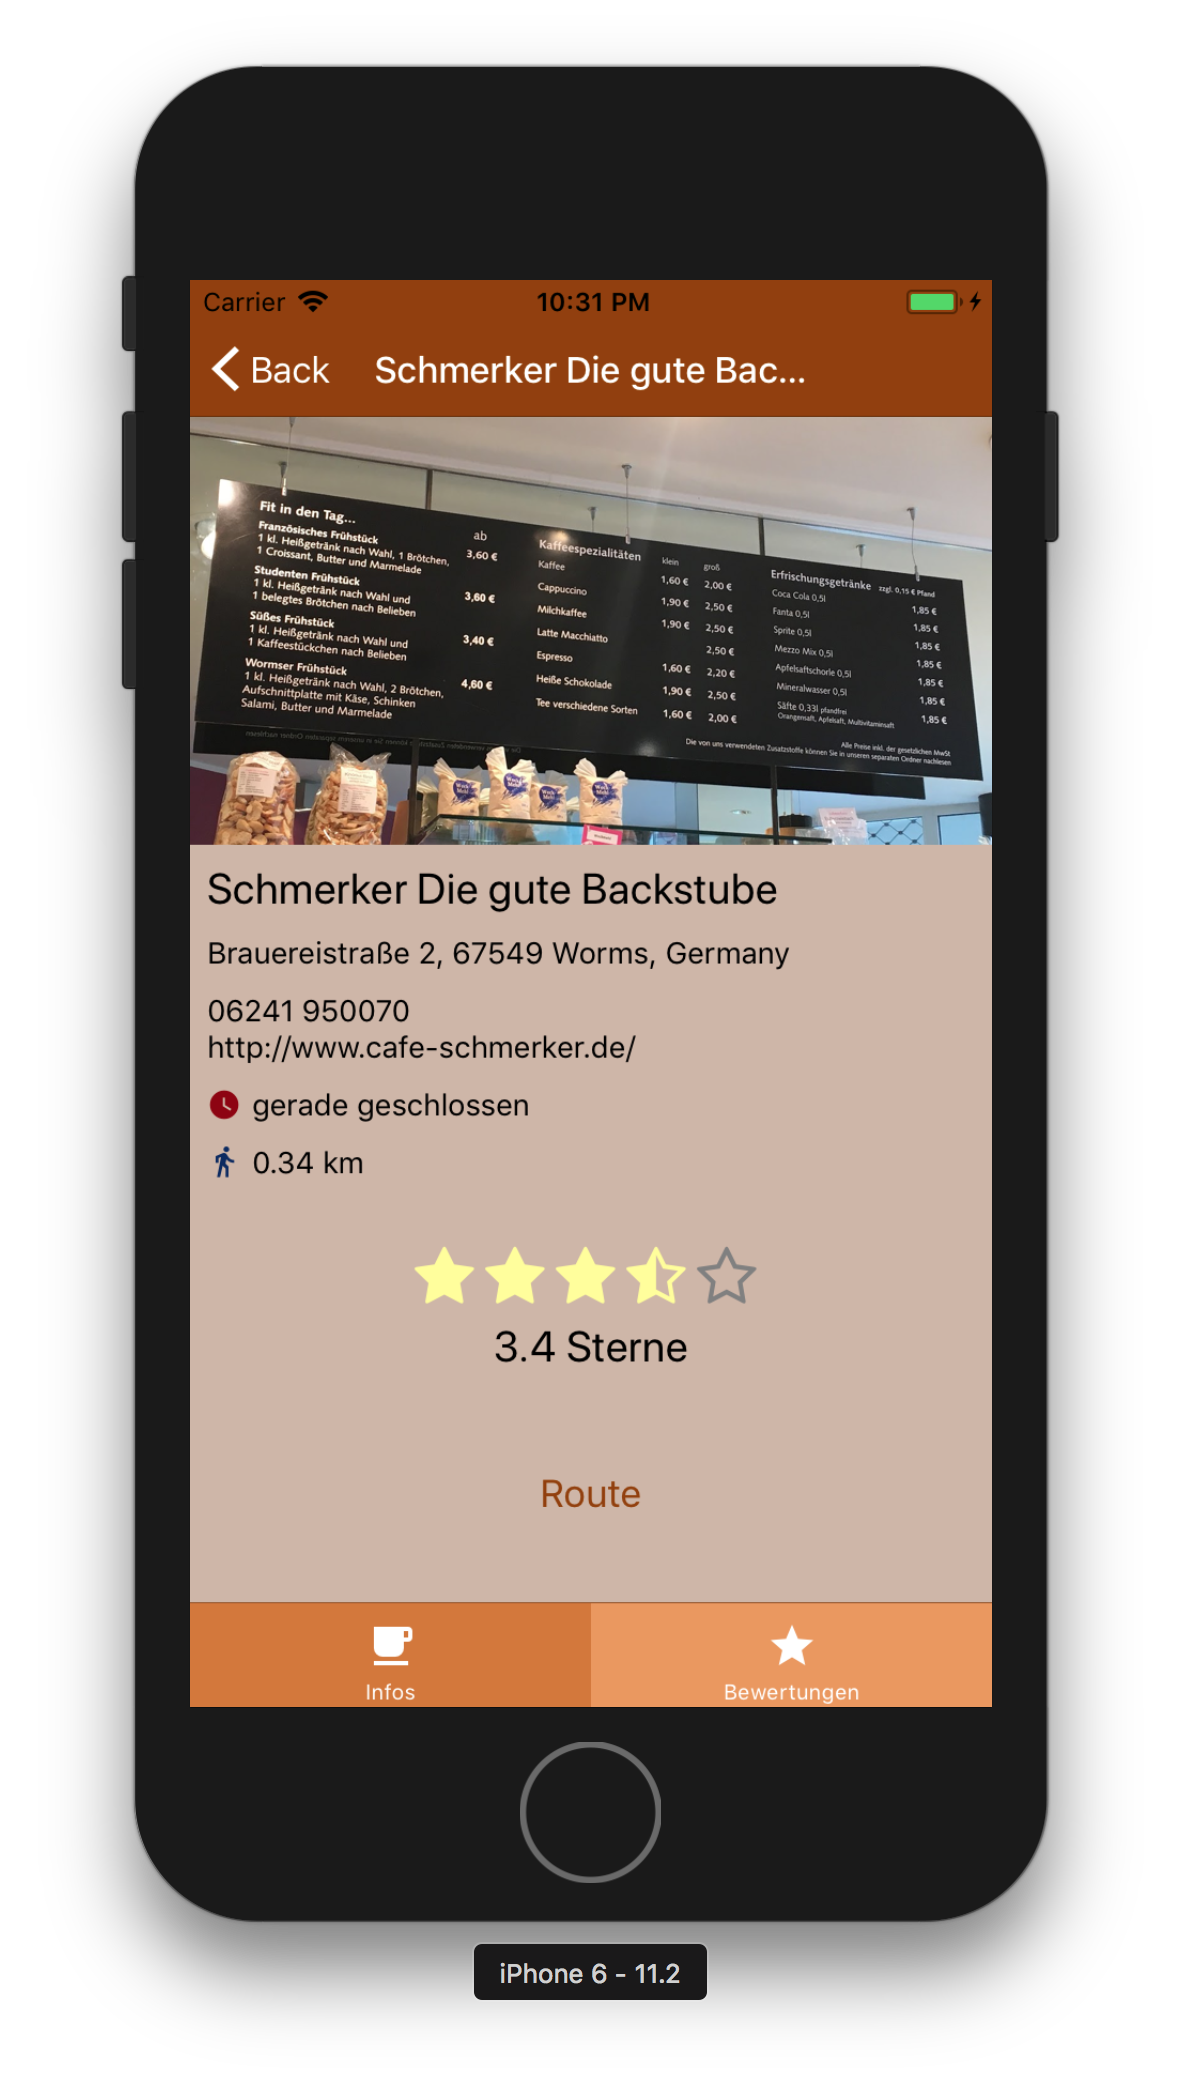
\includegraphics[width=0.5\textwidth]{Bilder/app-info.png}
		\captionof{figure}{Infoseite eines Cafés der App unter iOS} &
		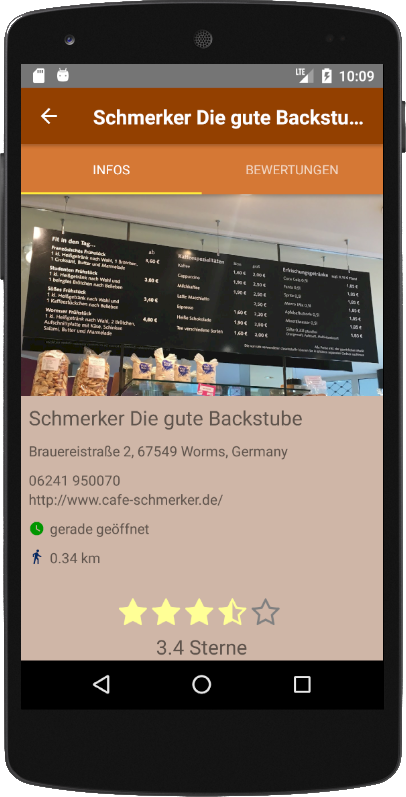
\includegraphics[width=0.5\textwidth]{Bilder/app-info_android.png}
		\captionof{figure}{Infoseite eines Cafés der App unter Android}
	\end{tabular}
\end{table}

\begin{table}
	\vskip-3.5cm\hskip-0.2cm\begin{tabular}{p{0.5\textwidth}p{0.5\textwidth}}
		\multicolumn{2}{p{\textwidth}}{\subsection{Bewertungen Café}} \\
		\multicolumn{2}{p{\textwidth}}{Alle über die Google API verfügbaren Bewertungen des ausgewählten Cafés werden hier in einer Liste angezeigt. Dabei erhält man Infos wie den Wert der abgegebenen Bewertung, den Zeitraum, den Berwertungsext sowie den Namen des Re­zen­senten.} \\
		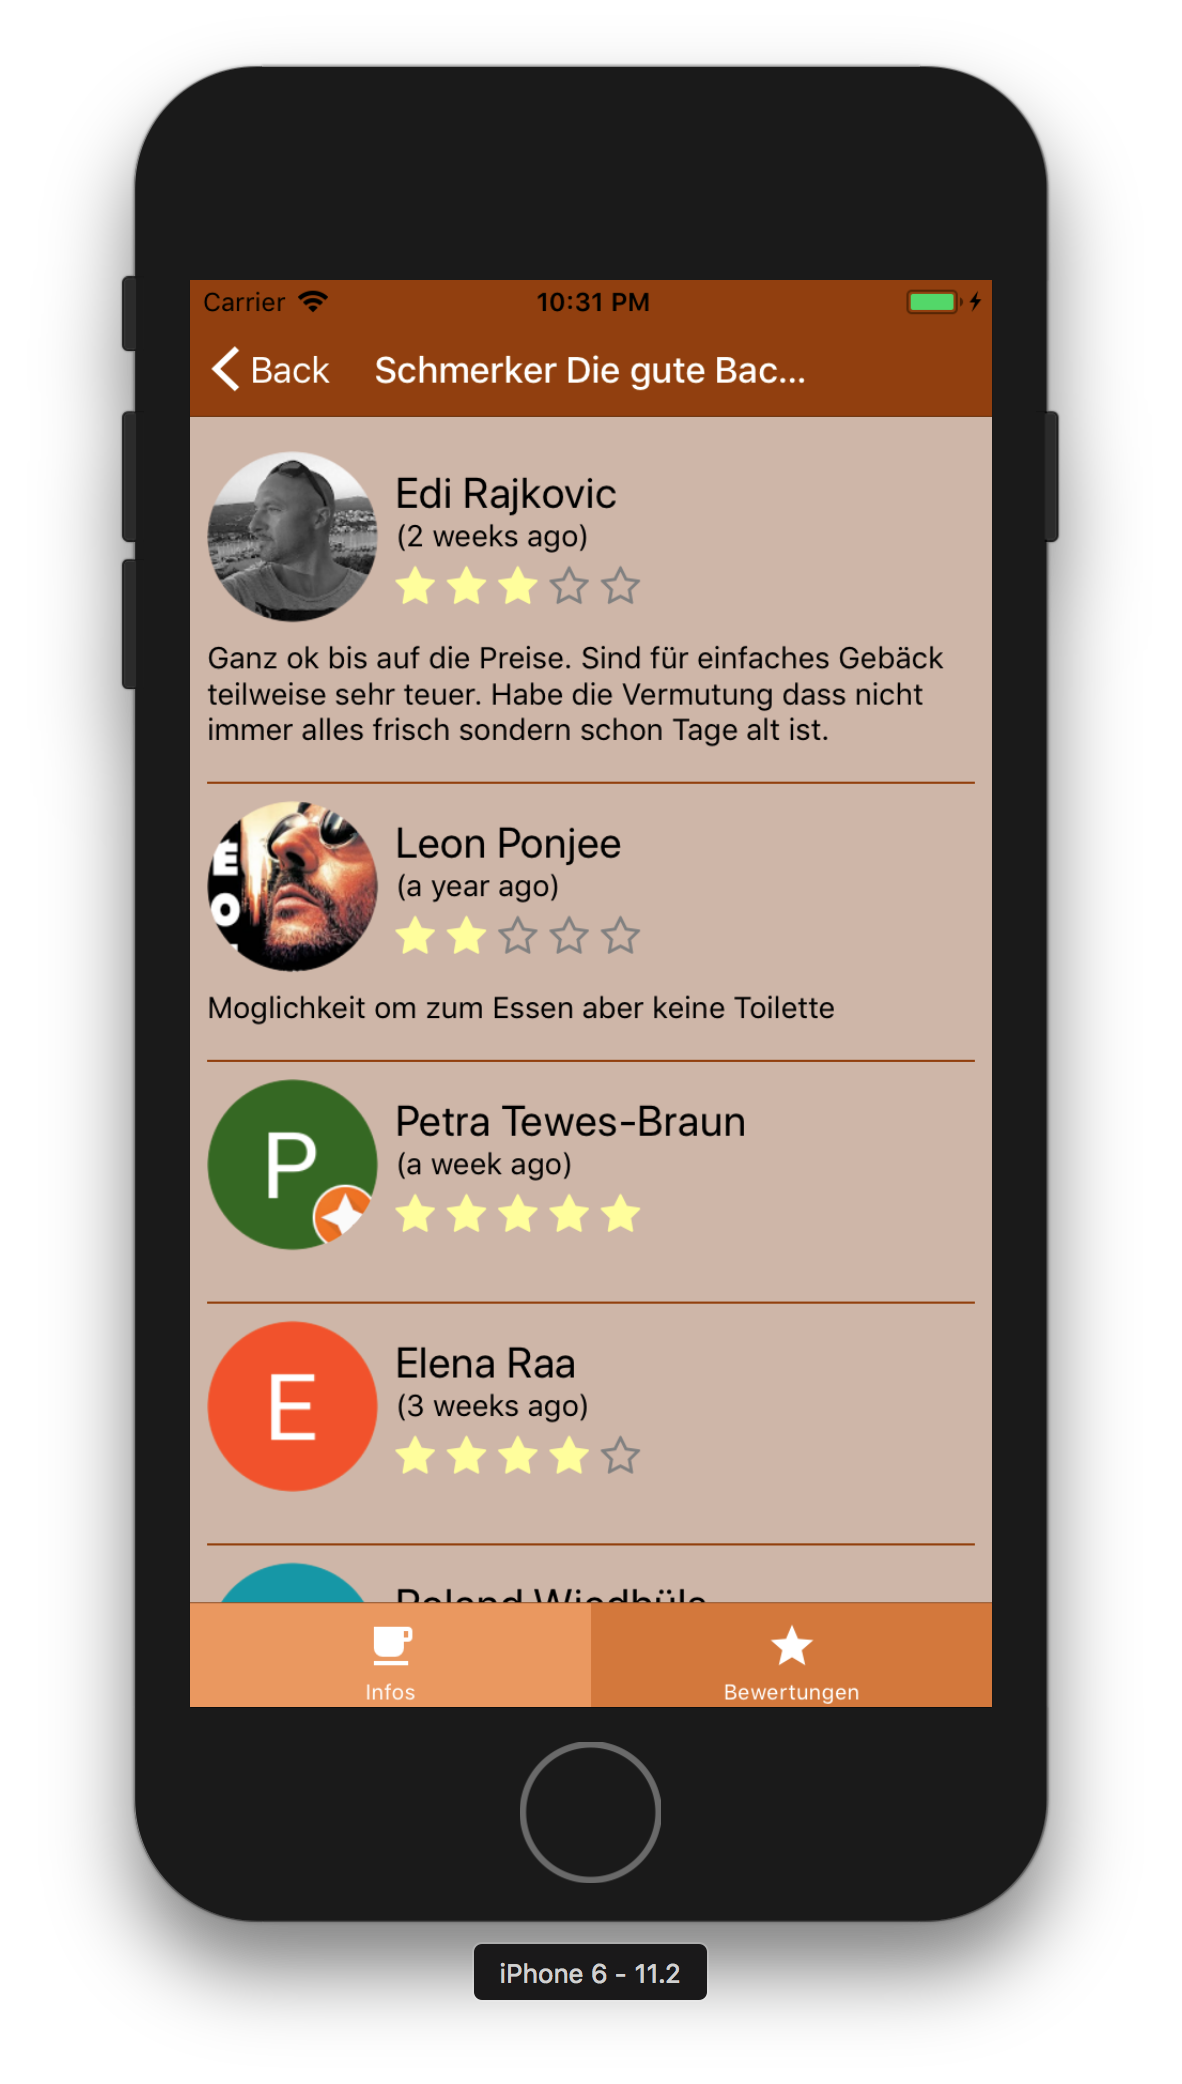
\includegraphics[width=0.5\textwidth]{Bilder/app-bewertungen.png}
		\captionof{figure}{Bewertungsseite eines Cafés der App unter iOS} &
		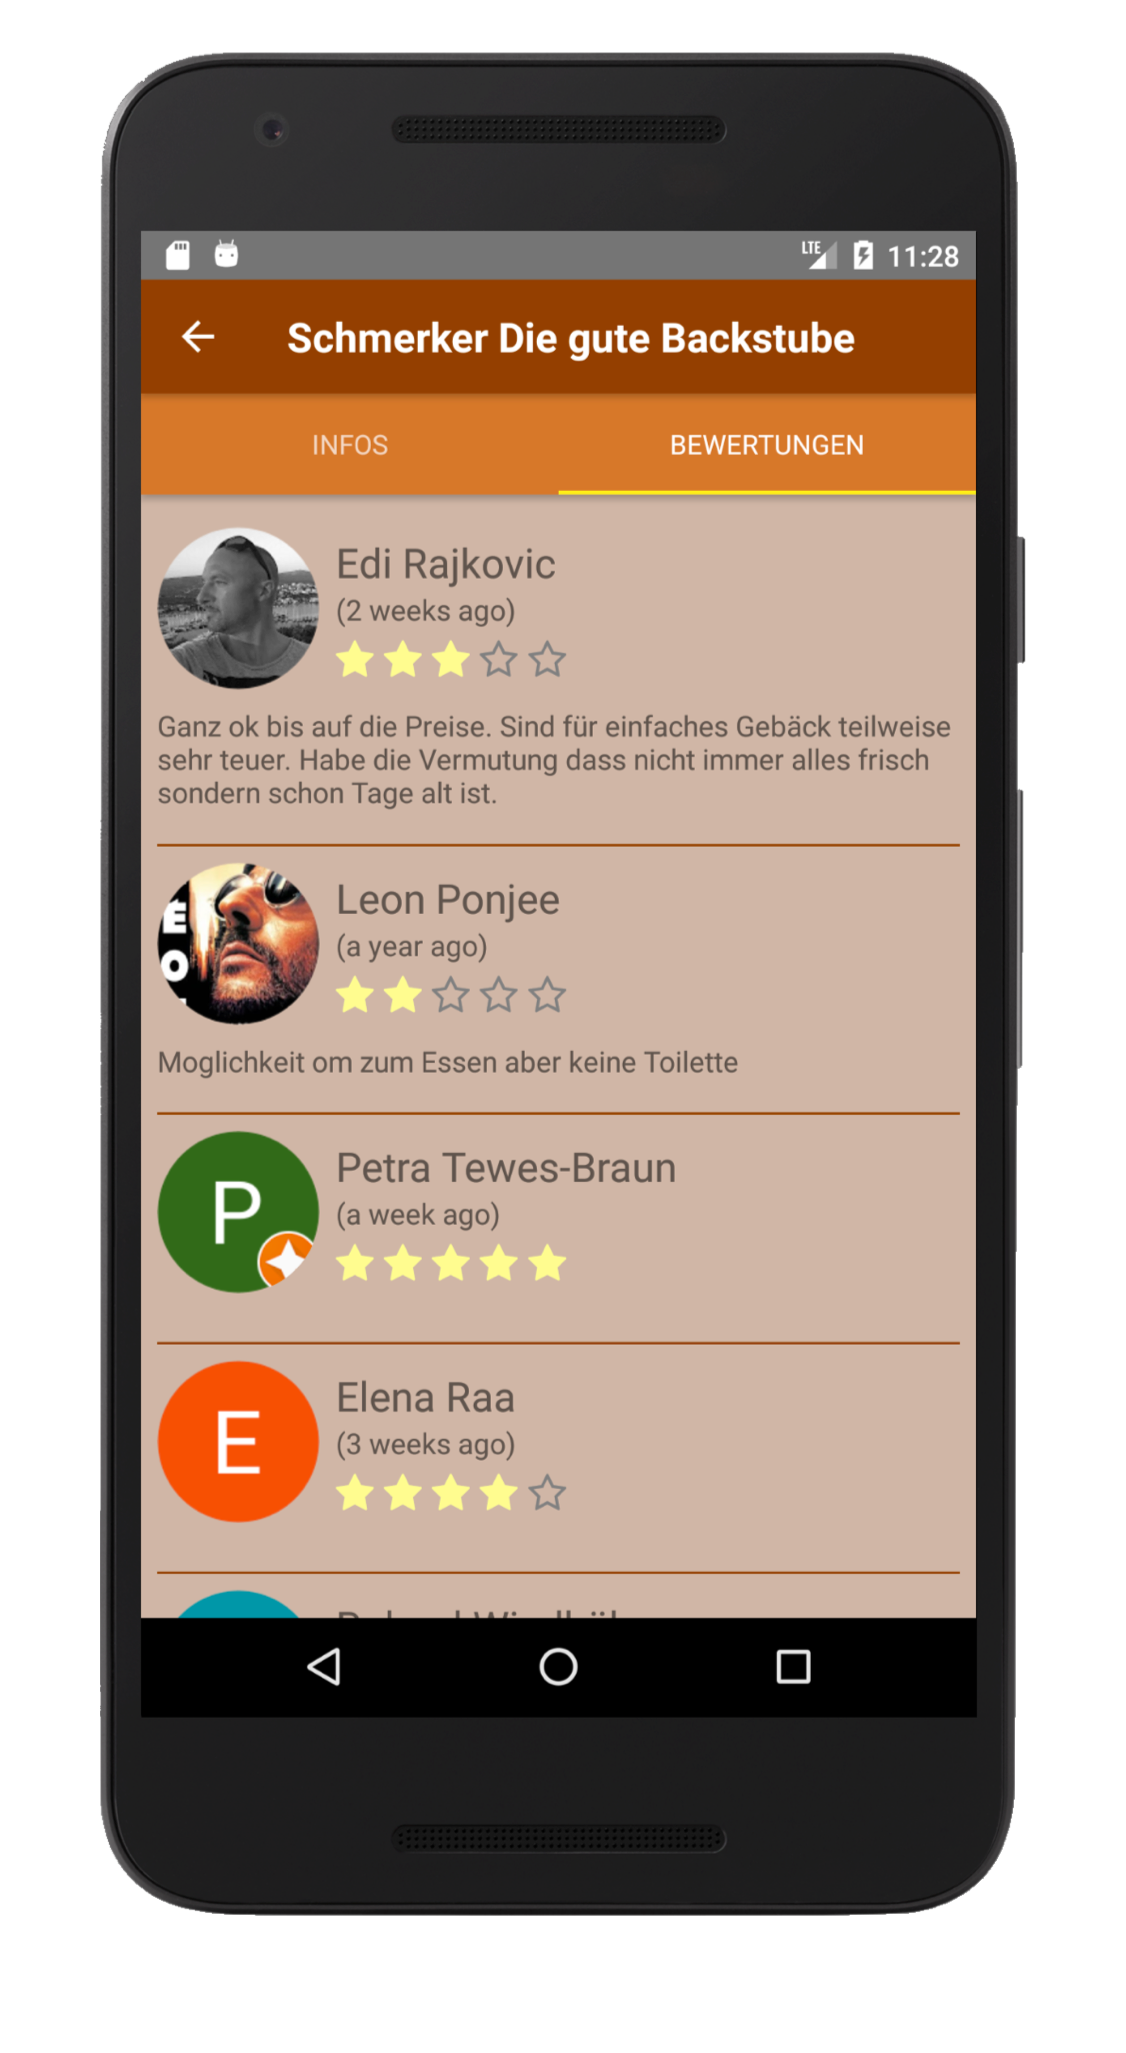
\includegraphics[width=0.5\textwidth]{Bilder/app-bewertungen_android.png}
		\captionof{figure}{Bewertungsseite eines Cafés der App unter Android}
	\end{tabular}
\end{table}

\begin{table}
	\vskip-2.5cm\hskip-0.2cm\begin{tabular}{p{0.5\textwidth}p{0.5\textwidth}}
		\multicolumn{2}{p{\textwidth}}{\subsection{Lexikon}} \\
		\multicolumn{2}{p{\textwidth}}{Die Übersichtsseite des Lexikons zeigt alle in der App hinterlegten Zubereitungsarten mit Namen und Icon. Ein Klick auf eines dieser Elemente führt auf die zugehörige Detailseite. Außerdem ist dies die einzige Seite, auf der der Bewegungssensor aktiv ist. Wird eine Schüttelgeste ausgeführt, so erhält man eine zufällig ausgewählte Zubereitungsart in einem Alert angezeigt. Von diesem aus kann man ebenfalls entweder direkt zur vorgeschlagenen Detailseite gelangen oder den Alert wieder entfernen.} \\
		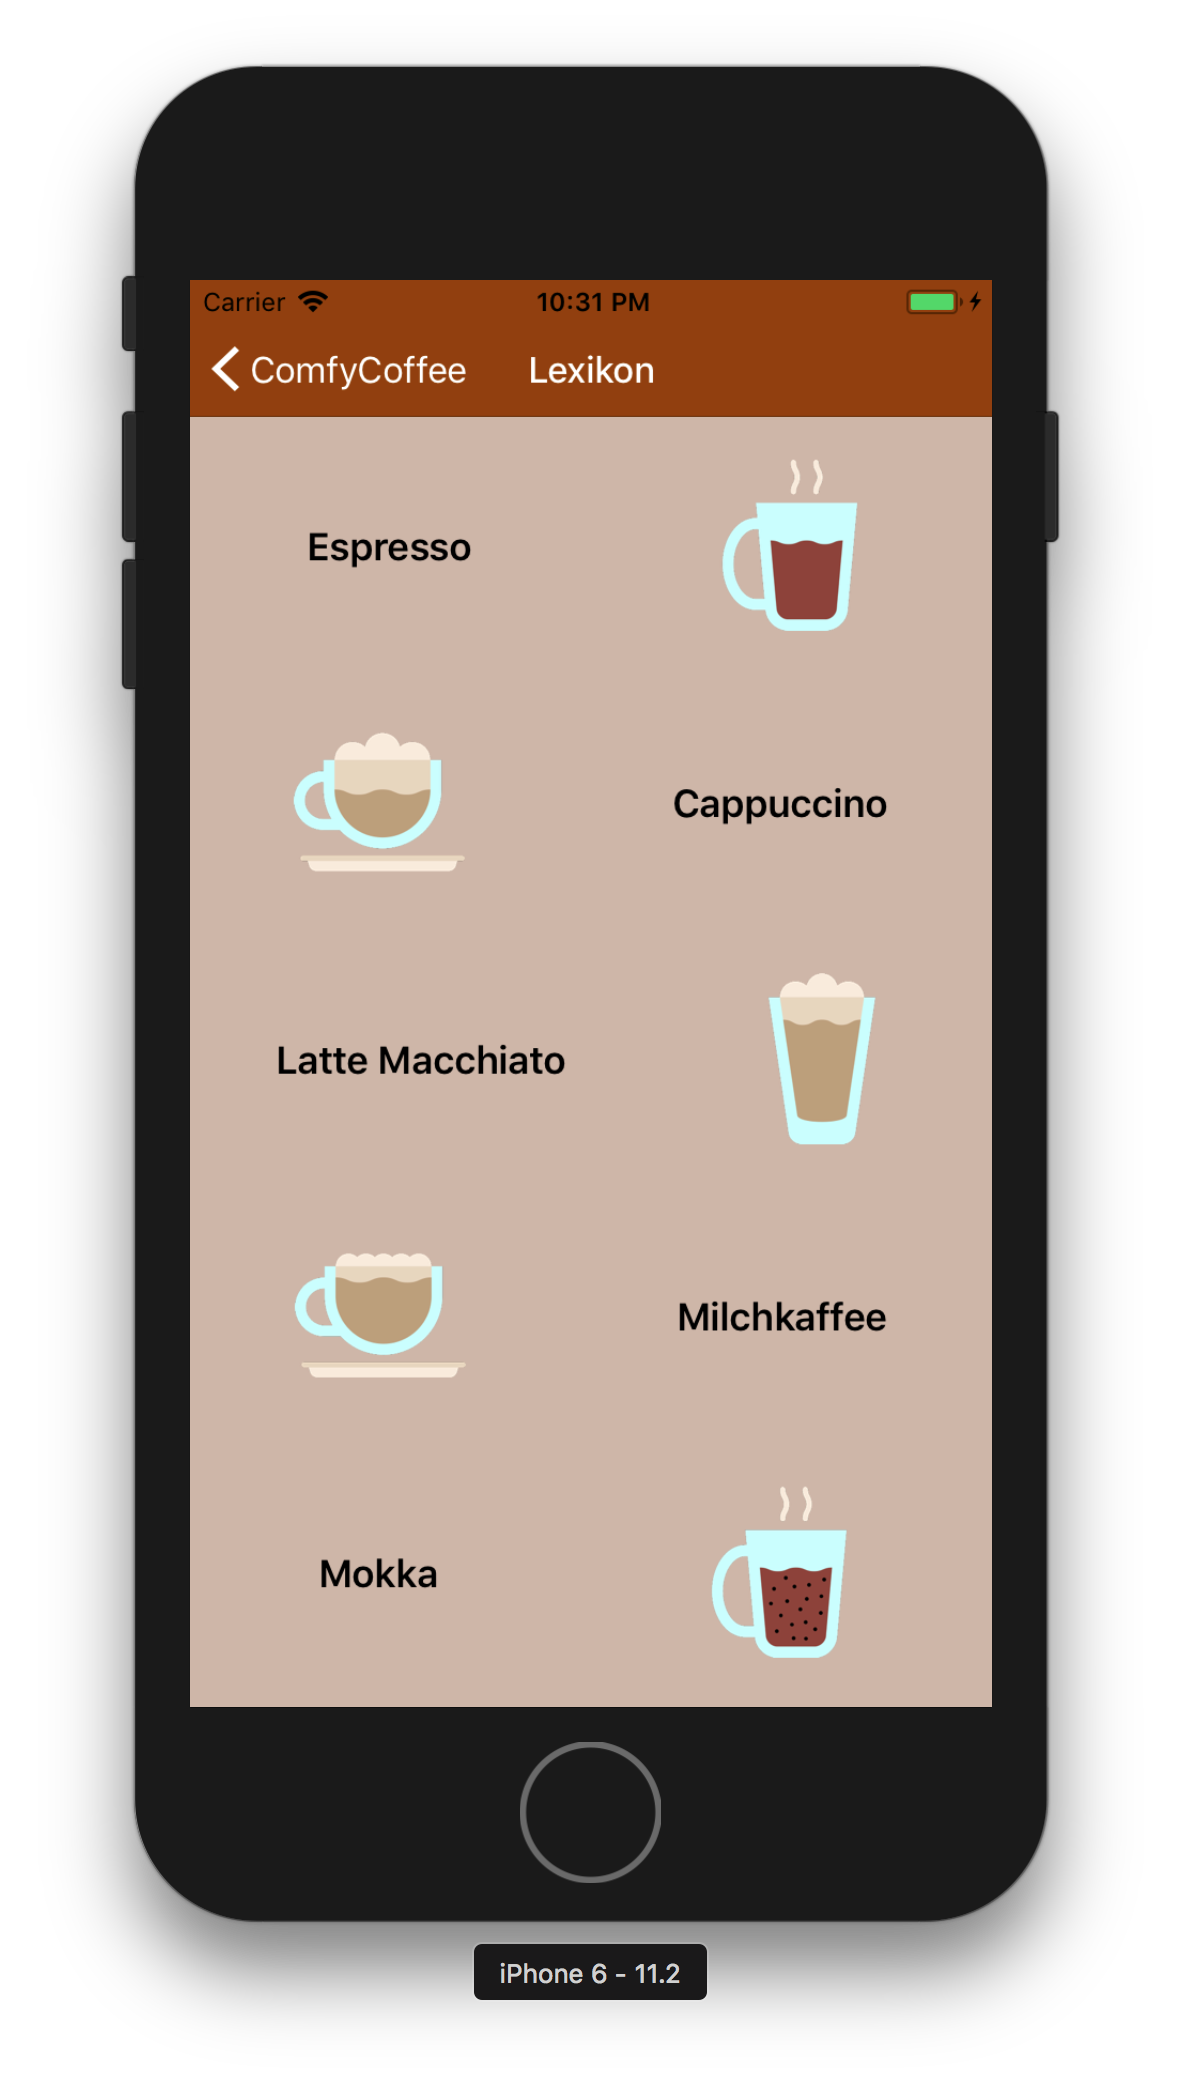
\includegraphics[width=0.5\textwidth]{Bilder/app-lexikon.png}
		\captionof{figure}{Lexikonseite der App unter iOS} &
		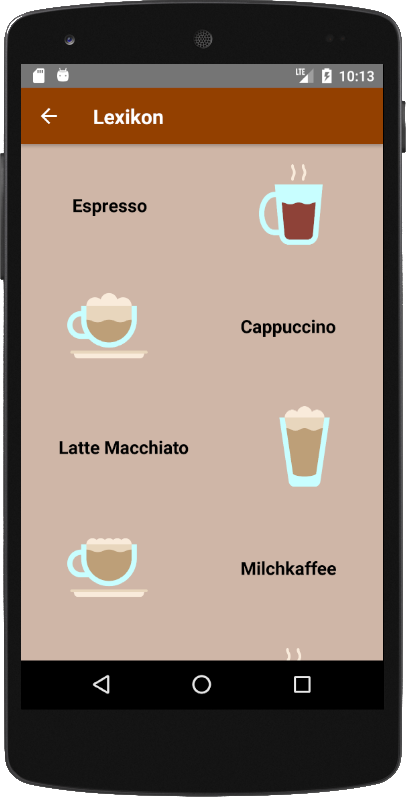
\includegraphics[width=0.5\textwidth]{Bilder/app-lexikon_android.png}
		\captionof{figure}{Lexikonseite der App unter Android}
	\end{tabular}
\end{table}

\begin{table}
	\vskip-2.5cm\hskip-0.2cm\begin{tabular}{p{0.5\textwidth}p{0.5\textwidth}}
		\multicolumn{2}{p{\textwidth}}{\subsection{Lexikon Detailansicht}} \\
		\multicolumn{2}{p{\textwidth}}{Hat man sich für eine Zubereitungsart entschieden erscheint das Template dieser Seite gefüllt mit den passenden Informationen. Dazu gehören der Name, das Icon, eine Beschreibung des Ablaufs sowie einige Attribute wie Stärke des Getränks oder Menge des benötigten Wassers. Diese Informationen sind an die jeweils ausgewählte Zubereitungsart angepasst.} \\
		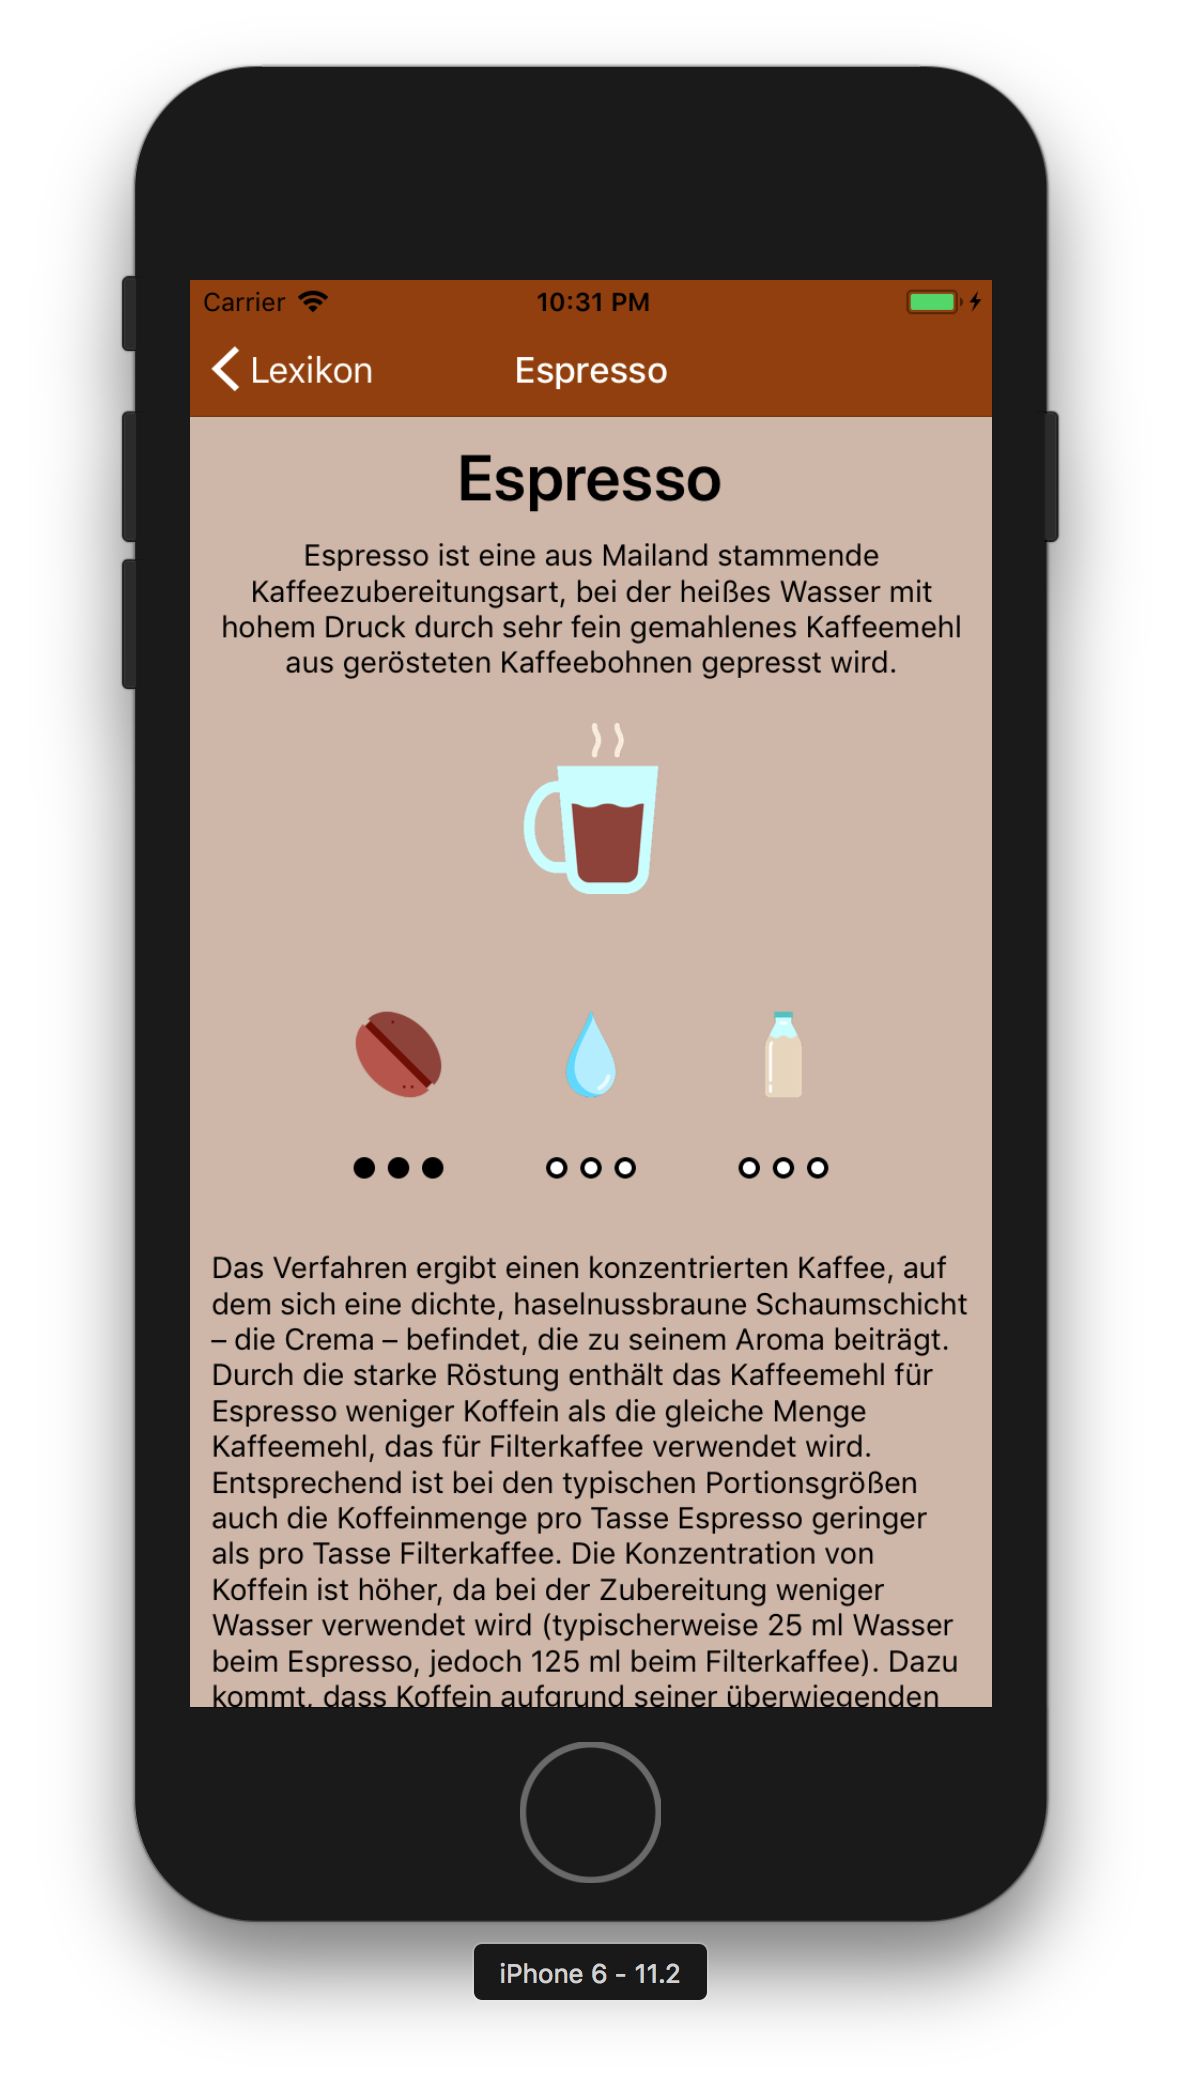
\includegraphics[width=0.5\textwidth]{Bilder/app-lexikon-detail.png}
		\captionof{figure}{Detailansicht eines Lexikoneintrags der App unter iOS} &
		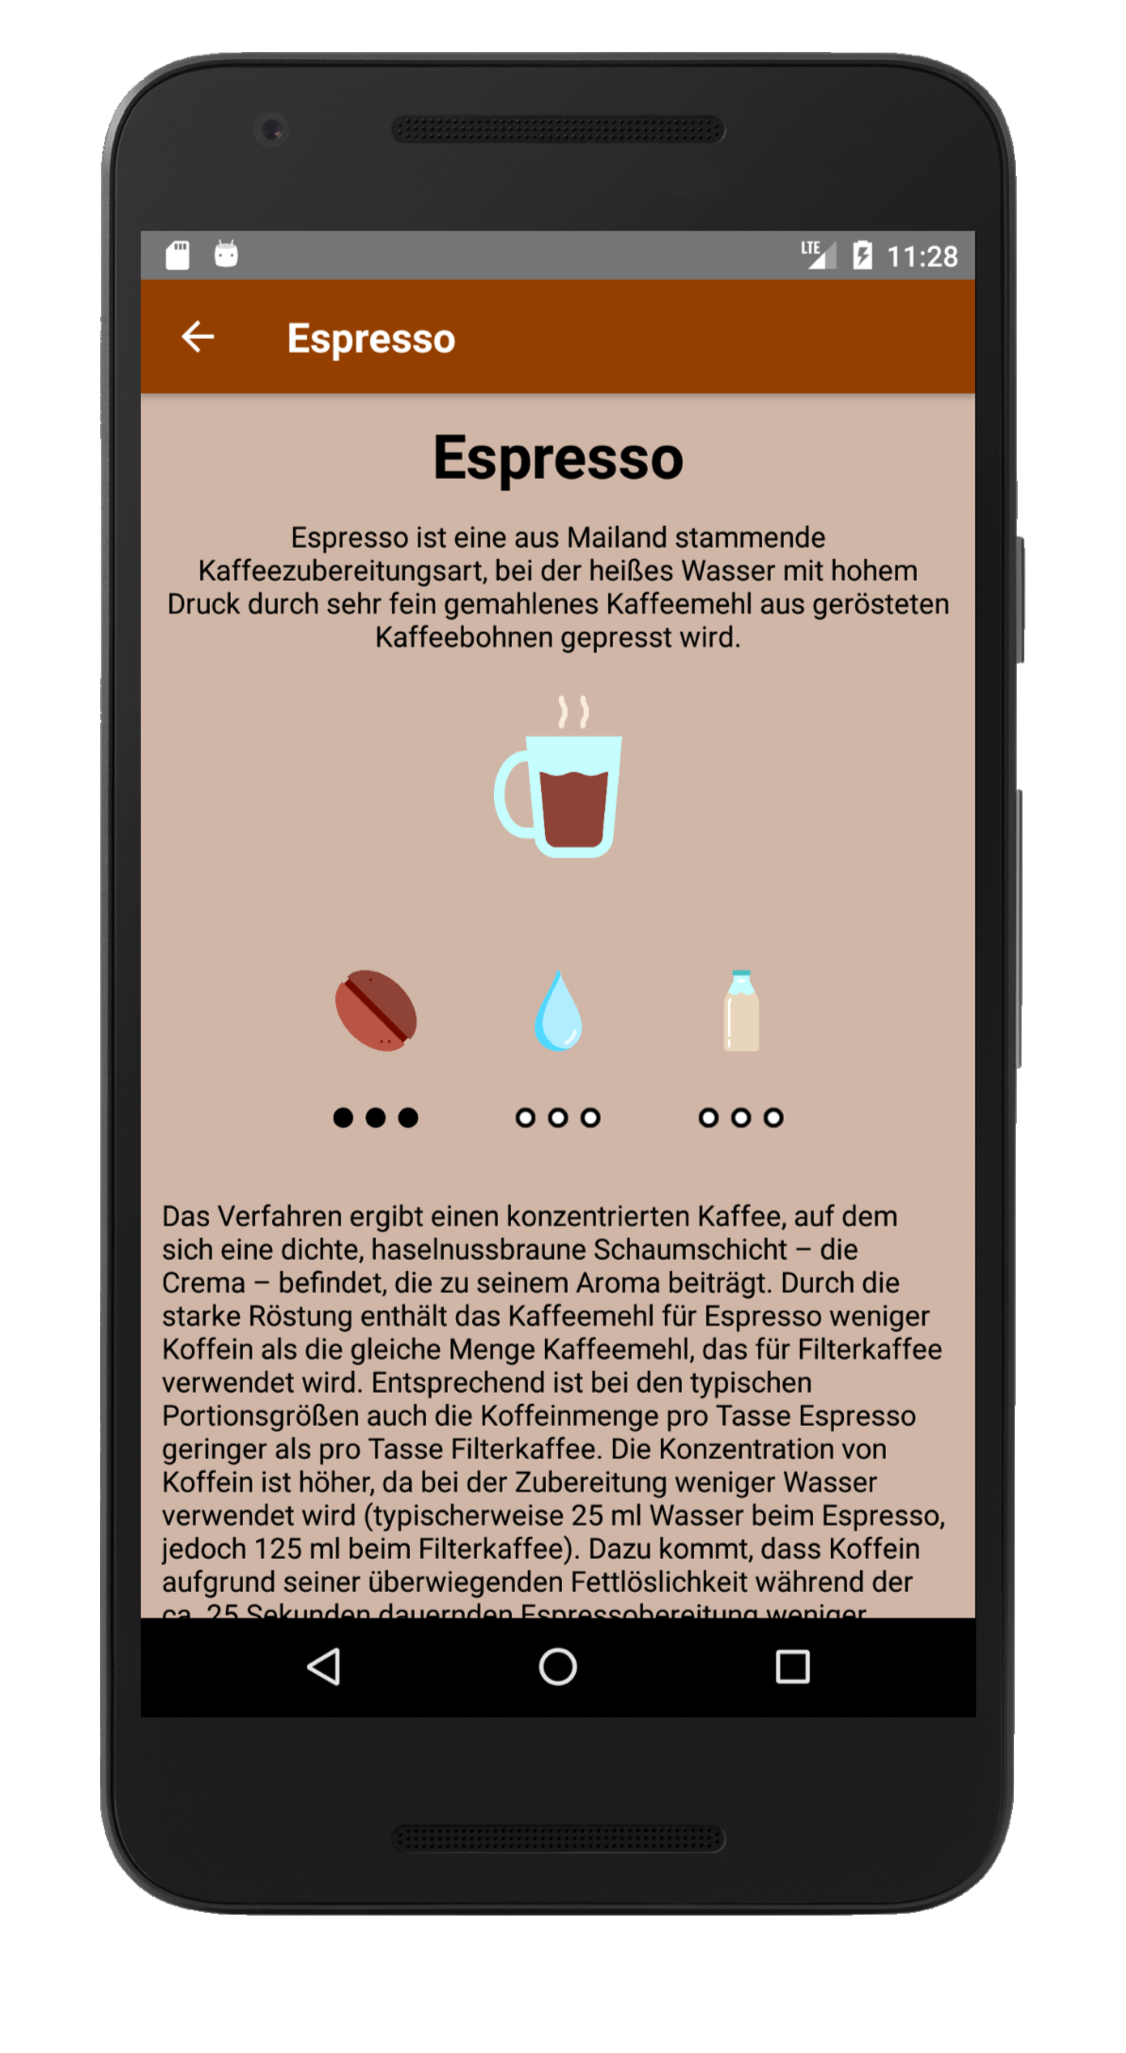
\includegraphics[width=0.5\textwidth]{Bilder/app-lexikon-detail_android.png}
		\captionof{figure}{Detailansicht eines Lexikoneintrags der App unter Android}
	\end{tabular}
\end{table}


\newpage

\section{Readme}
comfycoffee ist eine Cross-Plattform App zur Anzeige lokaler Cafés und damit nachhaltiger Unterstützung der lokalen Kaffeewirtschaft.
Das Repository ist öffentlich und unter folgendem Link erreichbar: https://bitbucket.org/codemeleon/comfycoffee
Weitere Informationen können der offiziellen React Native Dokumentation entnommen werden.

\subsection{Voraussetzungen}
Um an dem Projekt zu arbeiten müssen folgende Tools installiert sein:

\begin{itemize}
	\item node.js (v8.6.0 wird empfohlen)
	\item npm (v5.3.0 wird empfohlen)
	\item Watchman
	\item Xcode: (für iOS Builds - nur für MacOS)
	\item Android Studio: (for Anrdoid Builds)
	\item git
\end{itemize}

Es wird die Verwendung von \emph{Visual Studio Code (VS Code)} als Code Editor empfohlen.
Das VS Code Plugin \emph{Prettier - Code formatter} sorgt hierbei für einen sauber formatierten Code.


\subsection{Testing und Debugging}
Das Testing und Debugging kann über die in Android Studio und Xcode integrierten Simulatoren erfolgen.
Eine weitere Möglichkeit ist die direkte Verbindung zu einem Smartphone/iPhone über USB.
Wird ein derartiges Endgerät erkannt erfolgt die Kompilierung direkt auf das Gerät.

Relevante Befehle in der Kommandozeile sind hierbei:
react-native run-andoid
react-native run-ios

Hilfreiche Freatures wie JavaScript Debugging im Browser oder LiveReload können direkt im Simulator oder auf dem Endgerät aktiviert werden.


\subsection{Lizenz}
Das Projekt ist lizensiert unter der MIT Lizenz.







\chapter{Ausblick}
\label{ausblick}
Während und nach der Entwicklung sollen Tests sicher stellen, dass die App gut bedienbar ist. Das Testkonzept hierfür wird in Kapitel \ref{sec:testkonzept} erläutert.

Anschließend spielt das Marketing eine wichtige Rolle, um die App erfolgreich unter die Zielgruppe zu bringen. Ansätze und Ideen hierfür sind in Kapitel \ref{sec:marketing} dargelegt.

\section{Testkonzept}
\label{sec:testkonzept}
Das Testkonzept besteht aus einem \emph{Usability Test}, der zusätzlich ein \emph{Interview} und einen \emph{A/B-Test} beinhaltet.

Für den Usability Test werden 10 bis 20  Versuchsteilnehmer aus der Zielgruppe benötigt. Unter Beobachtung sollen sie die App bedienen und mit ihr bestimmte Aufgaben lösen. Währenddessen sollen die Teilnehmer laut aussprechen, was sie gerade denken und tun (\emph{Thinking Aloud}). So lassen sich unlogische Abläufe und unklare Bedienungen in der App herausfinden.

Das Interview wird als halb-strukturiertes Interview durchgeführt. Offene Fragen, die sich auf die App im Allgemeinen beziehen, lassen der Versuchsperson die Freiheit, ihre ganz persönlichen Eindrücke wiederzugeben. Diese Ergebnisse sind schwer zu vereinheitlichen und müssen mit entsprechender Umsicht behandelt werden, da sie sehr subjektive Empfindungen beinhalten, die sich unter Umständen nicht mit einem Großteil der Zielgruppe decken. Es muss stets abgewogen werden, ob und wie die Ergebnisse der offenen Fragen umgesetzt werden. Der geschlossene Teil des Interviews bezieht sich auf den A/B-Test im folgenden Abschnitt.

Beim A/B-Test wird ein Bestandteil der App in zwei unterschiedlichen Ausführungen getestet. Die Versuchspersonen werden in zwei Gruppen aufgeteilt, eine Gruppe erhält die App mit dem Bestandteil in der Version A, die andere die gleiche App, die sich nur darin unterscheidet, dass Bestandteil A durch B ausgetauscht wird. Im Fall von comfycoffee wäre zu testen, in welcher Form die Schüttelfunktion besser bei der Zielgruppe ankommt. Ursprünglich weist die Schüttelfunktion den Nutzer auf eine zufällige Kaffeesorte hin (vgl. Kapitel \ref{subsec:mussanforderungen}). Eine weitere Idee ist, über die Schüttelfunktion zufällig auszuwürfeln, wer von zwei oder mehreren Nutzern den Kaffee bezahlt. Präzise geschlossene Fragen sollen darüber Auskunft geben, welche Funktion von der Zielgruppe besser angenommen wird.

\section{Marketing}
\label{sec:marketing}
Beim Marketing wurden die Bereiche \emph{Produktpolitik}, \emph{Preispolitik}, \emph{Distributionspolitik}, \emph{Kommunikationspolitik} und \emph{Retention Marketing} ausgearbeitet.

\subsection{Produktpolitik}
Comfycoffee wird als App für Android und iOS entwickelt. Eine zusätzliche Web-App für Desktopnutzer ist denkbar.

\subsection{Preispolitik}
Comfycoffee wird als kostenfreier Download in den App-Stores zur Verfügung stehen. Cafés können einen höheren Platz in der Listenansicht der Cafés erkaufen, diese Einträge werden für den Nutzer kenntlich mit ``Anzeige'' markiert. Mit den Daten der Nutzer sowie der Cafés kann personalisierte Werbung innerhalb der App geschaltet werden.

Eine weitere Idee wäre, die App für einen geringen Preis in die App-Stores zu stellen. Dem Nutzer wird der Kauf schmackhaft gemacht, indem er Gutscheine von Cafés durch die App erhält, welche die Kosten für die App wieder aufwiegen.

\subsection{Distributionspolitik}
Die App wird in den App-Stores sowie über den Browser (Web-App) zur Verfügung gestellt.

\subsection{Kommunikationspolitik}
Eine dedizierte Landing-Page ist die erste Anlaufstelle für comfycoffee. Weitere Social Pages dienen eben diesem Zweck. Durch Social Media Werbung, besonders in ``Support your Locals''-Communities und durch Influencer, soll die Bekanntheit der App gesteigert werden.

Ein eigener Blog soll die Nutzer informieren und neue NUtzer gewinnen. Ein ``Kaffee-Reporter'' fungiert als Gesicht für die App und stellt Themen wie der ``Coffee of the Week'', die ``Location of the Week'' oder aktuelle Kaffee-Trends vor.

Offline-Werbung in Cafés vor Ort und Zeitungen machen die App auch in Kreisen bekannt, die weniger in den Soziale Medien unterwegs sind, bekannt.

\subsection{Retention Marketing}
Comfycoffee soll die Nutzer motivieren, die App regelmäßig zu nutzen. Hierfür können mit den Cafébesitzern, deren Cafés in der App aufgelistet werden, Gutscheine ausgehandelt werden, die die Nutzer über die App erhalten und einlösen können.

Die Nutzer können durch den Besuch ihres Lieblingscafés Punkte erhalten, anhand derer sie in einer Rangliste nach oben steigen können. Die Top 10 der Besucher des jeweiligen Cafés werden dort aufgelistet. Alternativ können die Nutzer Punkte erlangen, indem sie möglichst viele verschiedene Cafés besuchten. Durch diese Art der Gamification sollen die Nutzer Spaß an der App haben und diese durch den Ehrgeiz der Punktegewinnung möglichst oft nutzen.

Innerhalb der App kann auf bestimmte seltene Kaffeesorten aufmerksam gemacht werden, z. B. wenn sich der Nutzer gerade in der Nähe eines Cafés befindet, welches diese Sorte anbietet. Aktuelle Kaffee-Trends können zeitlich begrenzt in der App angesehen werden. Durch den Besuch eines Cafés können weitere Einträge im Lexikon freigeschaltet werden. Durch eine zeitliche Limitierung wird der Nutzer dazu aufgefordert, comfycoffee häufig zu nutzen.

\underline{Learnings:}
Auch nach der Entwicklung ist noch viel zu tun. Regelmäßiges Testen erhöht die Usability der App und bringt den Entwickler auf den Boden der Tatsachen zurück. Auch Marketing ist ein eigenes Themengebiet mit vielen Facetten, die es zu meistern gilt, um eine App wirkungsvoll unter die Zielgruppe zu bringen. Hier wird viel Einarbeitung und Ausdauer verlangt, um erfolgreich zu sein.
\chapter{Fazit}
\label{fazit}
Die Konzeption und Umsetzung einer Cross-Plattform-App war für uns Neuland, ebenso wie das Ausarbeiten eines Marketingkonzepts (vgl. Kapitel \ref{sec:marketing}). Im Folgenden sind unsere gewonnenen Erkentnisse und ein Fazit zum Entwicklungsframework React Native sowie der Cross-Plattform-Entwicklung im Vergleich zur nativen Entwicklung aufgeführt.

\section{Lessons Learned}
Comfycoffee war die erste Cross-Plattform App, die wir entwickelt haben. Auch mit dem Framework React Native haben wir unsere ersten Schritte gemacht (vgl. Kapitel \ref{sec:reactnative}). Dabei haben wir den Umgang mit APIs vertieft. Das Umsetzen von nativem Design in Android und iOS entsprechend den jeweiligen Design Guidelines birgt einige Herausforderungen. So haben Android und iOS teilweise die gleiche Bezeichnung für verschiedene Elemente, oder verschiedene Elemente mit dem gleichen Namen. Auch das Ansprechen von Hardwareschnittstellen (GPS, Bewegungssensor) war neu. Zu verstehen, wie diese funktionieren und benutzt werden können bedeutet oft viel lesen und, je nach Aussagekraft der Dokumentationen, noch mehr ausprobieren.

Herausforderungen waren auch gegeben bei der Benutzung eines weniger etablierten Frameworks wie React Native (vgl. Kapitel \ref{sec:reactnativefazit}).

Neu war außerdem die technische Konzeption mit der Implementierung der zuvor ausgearbeiteten, technischen Anforderungen. Die technische Konzeption steht der Produktkonzeption gegenüber, bei der Zielgruppen, Design und Testkontzept ausgearbeitet und Marktanalysen durchgeführt werden. Den teil der Produktkonzeption wurde schon in dem Modul Mobile Usability behandelt. Mit comfycoffee die Verbindung zwischen Produkt- und technischer Konzeption und Umsetzung herzustellen war eine spannende Herausforderung.

\section{React Native}
\label{sec:reactnativefazit}
Das Cross-Plattform Framework React Native schlägt die Brücke zwischen Web- und mobiler Entwicklung. Durch die eingesetzten Webtechnologien wie JavaScript fiel uns durch unsere Affinität zur Webentwicklung der Einstieg nicht schwer. Dennoch hat React Native einige Nachteile bei der Entwicklung. Das Debugging von CSS beispielsweise ist im Simulator nicht möglich. Weiterhin bestehen native Abhängigkeiten trotz der Cross-Plattform Eigenschaften des Frameworks. So mussten Libraries eingebunden und die Environment-Dateien separat per Hand konfiguriert werden. Es stehen online viele Module zur Erweiterung und Einbindung weiterer Elemente in React Native zur Verfügung, jedoch sind diese nicht immer ganz ausgereift oder gut dokumentiert.

\section{Cross-Plattform vs. Nativ}
Die Cross-Plattform Entwicklung mit React Native ist angelehnt an die Webentwicklung. Dies bietet gute Designmöglichkeiten dank CSS- und HTML-ähnlicher Strukturen. Der Hardwarezugriff ist dennoch gegeben und leicht anwendbar. Für eine kleine App wie ComfyCoffee wäre eine native Entwicklung für Android und iOS zu aufwändig gewesen. Die Vorteile der Cross-Platform Entwicklung - die Nutzung von Webtechnologien, die Designmöglichkeiten und der Hardwarezugriff - wiegen vor allem im Fall von comfycoffee die Nachteile auf. Die Entscheidung, womit eine App entwickelt werden soll, hängt zweifelsohne immer von den Anforderungen und Zielen der App ab. Wenn es machbar ist, würden wir jedoch lieber Cross-Platform bzw. hybrid statt nativ entwickeln.

\interlinepenalty = 10000

% Literaturverzeichnis ---------------------------------------------------------
%\bibliographystyle{apacite} % APA-Stil des Literaturverzeichnisses
%\bibliography{Bibliographie} % Aufruf: bibtex Diplomarbeit
%\nocite{*} % Bildet komplette Bibliographie ab

\addchap{Eidesstattliche Erklärung}

Hiermit versichere ich, dass ich die vorliegende Arbeit selbstständig und ohne Benutzung anderer als der angegebenen Hilfsmittel angefertigt habe. Alle Stellen, die wörtlich oder sinngemäß aus anderen Schriften entnommen wurden, sind als solche kenntlich gemacht.\\
Die Arbeit ist noch nicht veröffentlicht oder anderweitig für Prüfungszwecke vorgelegt worden.

\vspace{2\baselineskip}

Worms, den \einreichungsdatum

% Index ------------------------------------------------------------------------
%   Zum Erstellen eines Index, die folgende Zeile auskommentieren.
% ------------------------------------------------------------------------------
%\printindex

\end{document}